% !TEX program = xelatex
\documentclass[12pt,a4paper,UTF8,fontset=founder]{ctexart}

% === 中文支持 ===
% fontset=founder 使用方正书宋，覆盖最全的汉字字符集（包括所有罕见字）

% === 页面 ===
\usepackage[top=2.5cm, bottom=2.5cm, left=2.5cm, right=2.5cm]{geometry}
\usepackage{setspace}
\onehalfspacing

% === 表格 ===
\usepackage{booktabs}
\usepackage{longtable}
\usepackage{array}
\usepackage{threeparttable}
\usepackage{tabularx}

% === 图表 ===
\usepackage{graphicx}
\usepackage{caption}
\graphicspath{{figures/}}
\usepackage{float}

% === 数学 ===
\usepackage{amsmath,amssymb}

% === 超链接 ===
\usepackage[hidelinks]{hyperref}
\usepackage{xurl}  % 更好的 URL 换行

% === 页眉页脚 ===
\usepackage{fancyhdr}
\pagestyle{fancy}
\fancyhf{}
\fancyhead[L]{\small 《地书》图形语言的语言性量化评估}
\fancyfoot[C]{\thepage}
\renewcommand{\headrulewidth}{0.4pt}

% === 参考文献格式 ===
% Pandoc --citeproc 内联引用格式支持
\newlength{\cslhangindent}
\setlength{\cslhangindent}{1.5em}
\newlength{\csllabelwidth}
\setlength{\csllabelwidth}{3em}
\newenvironment{CSLReferences}[2]%
  {\begin{list}{}{%
    \setlength{\leftmargin}{0pt}%
    \setlength{\itemindent}{0pt}%
    \setlength{\itemsep}{0pt}%
    \setlength{\parsep}{0pt}%
    \setlength{\listparindent}{\parindent}%
    \setlength{\topsep}{0pt}}}%
  {\end{list}}
\newcommand{\CSLLeftMargin}[1]{%
  \leavevmode\par\noindent
  \makebox[\csllabelwidth][l]{#1}%
  \hspace{0pt}}
\newcommand{\CSLRightInline}[1]{%
  \parbox[t]{\dimexpr\linewidth-\csllabelwidth\relax}{#1}}

% === 标题信息 ===
\title{{\Large \textbf{《地书》图形语言的语言性量化评估}}\\[4pt]
       {\large ——基于多维标注体系的统计分析}}
\author{
  池长俊\thanks{人工智能与计算机学院，江南大学} \quad
  王顺祺 \quad
  刘棪 \quad
  高子阳}
\date{}

\begin{document}

\maketitle

% === 摘要 ===
\begin{center}
\begin{minipage}{0.92\textwidth}
\small
\setlength{\baselineskip}{1.6\baselineskip}
\textbf{摘\quad 要：}
图形符号系统（如Emoji、交通标志、UI图标）在当代数字通信中日益重要，但尚未有系统的计算框架来评估它们在多大程度上"像一种语言"。本文以徐冰《地书》为案例，提出一个多维度的"语言性"量化评估框架，涵盖频率结构、信息密度、词汇多样性、语法类别多样性、篇章结构复杂度和语义稳定性六个维度。基于708个标注文件中的46,494条语言学标注数据，对《地书》与八种自然语言语料库进行了系统对比。研究发现：（1）《地书》的词汇频率严格遵循齐夫幂律分布（R² = 0.923），但其Zipf斜率（$-$0.612）显著浅于中文自然语言（$-$1.35~$-$1.47），表明词频分布异常平坦；（2）在同等语料规模下，其词汇丰富度（降采样TTR = 0.434）约为中文的3倍，归一化熵（0.914）在所有对比语料中最高；（3）其语法类别分布呈现标点/边界标记主导（33.3\%）、动词性超过名词性（1.63:1）、虚词/语法标记极度稀缺（0.9\%）的三重特征；（4）篇章结构以时间先后为主线（43.7\%），复杂逻辑关系不足11\%。综合来看，《地书》在统计结构上遵循人类语言的深层组织规律，但其词汇分布模式反映了一个缺乏语法化功能词体系的符号系统所面临的系统性约束。本文据我们所知首次为图形符号系统提供了一套可复用的多维度语言性评估方法，并将标注者间分歧重新定位为揭示符号系统固有歧义性的研究窗口。
\end{minipage}
\end{center}

\vspace{0.3cm}

\begin{center}
\begin{minipage}{0.92\textwidth}
\small
\textbf{关键词：}地书；图形语言；语言性评估；标注者间一致性；齐夫定律；计算语言学
\end{minipage}
\end{center}

\vspace{0.5cm}

\begin{center}
\small
\textbf{English Title:} A Quantitative Language-ness Assessment of EarthScript (Di Shu):\\
Statistical Analysis Based on a Multi-Dimensional Annotation Framework
\end{center}

\newpage

% === 正文 ===

\section{引言}\label{ux5f15ux8a00}

\subsection{研究背景}\label{ux7814ux7a76ux80ccux666f}

人类对''普天同文''的想象几乎与文字本身一样古老。从莱布尼茨设想用数学符号构建''通用字符''（\emph{Characteristica Universalis}），到柴门霍夫创造世界语（Esperanto），再到 Otto Neurath 用图形符号设计''无边界语言''ISOTYPE------这一理想的核心冲动从未改变：\textbf{是否存在一种沟通系统，可以绕过自然语言的巴别塔，让所有人都能''读懂''？}

中国当代艺术家徐冰的《地书》（\emph{Book from the Ground}, 2003--）是这一传统中最近的、也可能是最系统的实践。徐冰从世界各地收集了数千个公共标识符号------机场图标、洗手间标志、交通指示、Emoji------用它们''书写''了一本没有任何传统文字的叙事书，讲述了城市白领''黑先生''24小时的生活。《地书》已在多个国家和地区出版，据称''无须翻译''即可阅读\textsuperscript{{[}1{]}}。徐冰还开发了配套的''地书字库''软件，可将中文或英文自动转译为对应的图形符号\textsuperscript{{[}2{]}}。

从语言学视角来看，《地书》提出了一个令人着迷的问题：\textbf{如果一种''语言''完全由图形符号构成------没有语音、没有字母、没有线性书写的语法标记------它在什么意义上还是一种''语言''？} 或者说，它在多大程度上具备自然语言的语言学属性？

这个问题并非仅仅关乎一件艺术作品。在当代数字通信中，图形符号系统正以前所未有的速度和规模渗透进日常语言实践------Emoji 每年新增数百个符号，全球数十亿人每天都在使用图形来补充、替代或修饰文字文本。理解图形符号系统的语言学属性，已经从一个理论好奇演变为一个具有实践意义的研究议题。

\subsection{研究空白与研究问题}\label{ux7814ux7a76ux7a7aux767dux4e0eux7814ux7a76ux95eeux9898}

然而，关于《地书》的现有学术研究几乎全部来自当代艺术、符号学和翻译学领域，采用的是定性分析方法\textsuperscript{{[}1--6{]}}。这些研究讨论了《地书》的''普天同文''声称、其符号学悖论、其与 ISOTYPE 的历史关联、其背后的政治符号学------但一个基本的问题从未得到系统回答：\textbf{从计算语言学的角度来看，《地书》到底有多''像''一种语言？}

这个空白的背后，是一个更一般性的方法论缺口：我们缺少一套系统性的工具和框架，用来量化评估一个非自然语言的符号系统在语言学维度上的''语言化''（language-ness）程度。

本文试图填补这两个空白。我们提出以下研究问题：

\begin{itemize}

\item
  \textbf{RQ1（描述性问题）}：在词频分布、信息量、语法类别、篇章结构、形态特征等维度上，《地书》与自然语言的统计模式有何异同？
\item
  \textbf{RQ2（方法论问题）}：能否设计一套可复用的量化评估框架，系统评估任意符号系统的''语言性''（language-ness）？
\item
  \textbf{RQ3（深度分析问题）}：多标注者的语言学判断在哪些维度、哪些语义类型上产生分歧？这些分歧揭示了图形语言的哪些系统性属性？
\end{itemize}

\subsection{研究设计与贡献}\label{ux7814ux7a76ux8bbeux8ba1ux4e0eux8d21ux732e}

为回答上述问题，本文采用了以下研究设计：

\textbf{数据基础}：基于一套专门为《地书》开发的多维度语言学标注体系（版本 \texttt{dishu\_cl\_nlp\_full\_v2}），该体系涵盖 10 个语言学维度------字面对应词（Literal Gloss）、词性类别（POS-like Category）、核心语义角色（Core Semantic Role）、类形态特征（Morphological Features）、语义基元（Semantic Primitives）、篇章关系（Discourse Relation）、言语行为（Speech Act）、语境实际含义（Pragmatic Meaning）、歧义来源（Ambiguity Sources）和视觉线索（Visual Cues）。来自多个标注者的 708 个文件、46,494 条标注构成了本文的分析基础。此外，21 个自然语言语料库（4 类中文体裁 + 16 种语言 Wiki）提供对照基线。

\textbf{分析框架}：本文提出一个六维度''语言性''量化评估框架，涵盖频率结构（D1）、信息密度（D2）、词汇多样性（D3）、语法类别多样性（D4）、篇章结构复杂度（D5）和语义稳定性（D6）。每个维度对应一个可计算的量化指标，并与自然语言的参考范围进行比较。

\textbf{分析工具}：本文运用了 Transformer 出现之前计算语言学的经典方法------齐夫定律拟合（Zipf's Law）、Shannon 信息熵、词汇丰富度指标（TTR/RTTR）、标注者间一致性系数（Fleiss' κ）------对《地书》与自然语言进行系统对比。

本文的贡献包括：

\begin{enumerate}
\def\labelenumi{\arabic{enumi}.}

\item
  \textbf{方法论贡献}：提出了一套可复用的图形符号系统''语言性''量化评估框架，该框架不限于《地书》，可应用于 Emoji、交通标志、UI 图标等任意符号系统的语言属性评估。
\item
  \textbf{实证贡献}：基于 46,000 余条标注数据，首次对《地书》进行了系统性的计算语言学定量分析------这是迄今为止对一个系统性图形语言最全面的统计刻画。
\item
  \textbf{理论贡献}：通过实证数据对话 Miton 和 Morin\textsuperscript{{[}7{]}} 的''像似性破坏效率''假说，提出了''像似性改变效率定义''的修正观点；通过对标注分歧的系统量化，将标注者间一致性从''质量控制指标''重新定位为''图形符号固有歧义性的研究窗口''。
\end{enumerate}

\subsection{论文结构}\label{ux8bbaux6587ux7ed3ux6784}

本文其余部分组织如下：第 2 章回顾《地书》研究、图形语言研究和统计语言学普遍规律的相关文献，明确研究空白；第 3 章详细描述标注体系、数据集和分析方法，介绍六维度语言性评估框架和歧义热力图的构建方法；第 4 章报告词频分布、词汇多样性、语法类别、篇章结构和形态特征五个维度的实证结果；第 5 章讨论这些发现的含义------地书在哪些维度上接近自然语言、在哪些维度上偏离，以及背后可能的语言学机制；第 6 章总结主要发现、研究贡献、框架的可扩展性和研究局限。

\newpage

\section{相关工作}\label{ux76f8ux5173ux5de5ux4f5c}

\subsection{《地书》及其现有研究}\label{ux5730ux4e66ux53caux5176ux73b0ux6709ux7814ux7a76}

徐冰的《地书》（\emph{Book from the Ground}）创作始于 2003 年，历时十余年完成。与他的《天书》（1987--1991，以自创的''伪汉字''解构文字的可读性）和《英文方块字》（1994--，将英文字母重组为汉字结构）一脉相承，《地书》用从世界各地收集的公共标识符号书写了一个无须翻译即可''阅读''的叙事------城市白领''黑先生''的 24 小时生活\textsuperscript{{[}1,3{]}}。徐冰还开发了配套的''地书字库''软件，可将中文或英文输入自动转译为对应的标识符号，在技术上构成了当代 Emoji 自动补全系统的艺术先声\textsuperscript{{[}2{]}}。

然而，现有对《地书》的学术研究几乎全部来自当代艺术、符号学和翻译学领域，采用的是\textbf{定性分析}方法。Lee\textsuperscript{{[}1{]}} 从翻译学视角分析了《天书》与《地书》对语言沟通的不同态度------前者表达了对文字传达可能性的消极怀疑，后者则展望了一个视觉符号功能替代文字的未来，并提出了''翻译性文本''（translational text）的概念框架。Teo\textsuperscript{{[}4{]}} 将《地书》置于中国互联网审查与底层视觉抵抗的政治语境中，讨论了其''普天同文''理想暗含的政治符号学张力，并将《地书》与 Otto Neurath 的 ISOTYPE 系统关联比较。Mersmann\textsuperscript{{[}2{]}} 将《地书》视为''通用图标文字''（universal icon writing），分析了数字时代''文字的图像转向''（iconic turn of writing）以及地书字库软件作为翻译装置的意义。中文符号学界，胡易容\textsuperscript{{[}5{]}} 从索绪尔和艾科的符号学框架出发，指出了《地书》``普天同文''声称中的核心悖论：那些看似''直观''的图标------心形代表爱、裙子代表女人------实质上是现代社会心理约定的产物，而非真正的普世通用符号。这回应了艾科\textsuperscript{{[}8{]}} 关于''任何看似像似的符号都是社会约定结果''的论断。Wang\textsuperscript{{[}6{]}} 以《地书》为案例进行了数字媒体艺术的符号叙事研究。

\textbf{研究空白}。上述研究共同构成了对《地书》的深厚定性理解，但一个显著的方法论空白仍然存在：\textbf{迄今为止，没有任何研究对《地书》进行过系统性的计算语言学定量分析}。其词频分布是否遵循齐夫定律？其信息熵与自然语言相比如何？其语法类别的分布结构具有什么特征？这些问题的答案------无论结果如何------都将为关于图形语言''语言属性''的理论讨论提供第一种量化证据。

\subsection{图形语言与视觉符号系统}\label{ux56feux5f62ux8bedux8a00ux4e0eux89c6ux89c9ux7b26ux53f7ux7cfbux7edf}

在《地书》之前和之后，人类对系统性图形沟通系统的探索从未停止。两个重要的前驱系统为理解《地书》提供了历史语境。

\textbf{Blissymbolics 与 ISOTYPE}。Charles K. Bliss 的 \emph{Semantography}（Blissymbolics，1949）是最早尝试构建系统性图形''文字''的方案之一，包含视觉动词、复合图标、限定词和代词等语法元素，采用组合逻辑生成新意义（如 pen + man = writer）。实证研究表明其符号具备低透明度（难以猜测）但高可解释性（解释后易学）的特征------在肯尼亚儿童的多语言实验中得到了验证。Otto Neurath 的 ISOTYPE（International System of Typographic Picture Education，1925--1934）则更侧重于信息可视化而非叙事性书写，但其''无边界语言''的理想与《地书》的''普天同文''追求一脉相承。计算符号学领域，有研究者以 Blissymbolics 为灵感，提出了基于语义网络和概念混合的计算符号自动生成系统，将位置、颜色和形状作为符号学维度进行了形式化探索。

\textbf{Emoji 语言学}。2010 年代后，Emoji 成为计算语言学中研究图形符号最活跃的对象，其方法论对本研究具有直接参照意义。近年来的关键进展包括：（1）Scheffler 等\textsuperscript{{[}9{]}} 对全部 107 个面部 Emoji 进行了效价、唤醒度、熟悉度、清晰度和视觉复杂度五维度标准化评分，复现了词汇研究中的效价-唤醒度 U 型关系，为 Emoji 作为''类词汇''单位提供了心理语言学证据；（2）Shardlow 等\textsuperscript{{[}10{]}} 证明了 Emoji 的多义性，构建了带 WordNet 义项标签的推文语料库，Emoji 义项预测达到平均路径相似度 $0.4146$；（3）Yang 等\textsuperscript{{[}11{]}} 在 LREC-COLING 2024 发布的 ELCo 数据集涵盖 209 个概念，发现简单策略（直接表征、重复）适用于具象概念，但抽象概念的图形表达需要隐喻组合------当前模型（包括 ChatGPT）在零样本设置下难以处理这类隐喻组合。这一发现与《地书》表达抽象概念的根本挑战高度对应。

\textbf{局限与本文的定位}。Emoji 语言学已建立了图形符号的计算分析范式，但其研究定位存在一个关键限制：Emoji 几乎总是被作为自然语言文本的\textbf{附加成分}来研究（Emoji+文字的情感分析、消歧等），而非作为一个\textbf{独立的符号系统}。本文的独特定位在于：将《地书》视为一个自足的图形语言系统，在多个语言学维度上直接与自然语言进行统计对比，而非研究它''辅助''自然语言的方式。

\subsection{统计语言学普遍规律与视觉系统}\label{ux7edfux8ba1ux8bedux8a00ux5b66ux666eux904dux89c4ux5f8bux4e0eux89c6ux89c9ux7cfbux7edf}

本文的研究设计深度依赖于统计语言学的两个核心理论------齐夫定律与信息熵------以及它们近年在视觉/图形系统中的验证研究。

\textbf{齐夫定律}（Zipf's Law）\textsuperscript{{[}12{]}} 指出，在自然语言中，词的频率与其排名呈反比关系：排名第 n 的词的出现频率约等于排名第 1 的词的 1/n。在双对数坐标上，这表现为一条斜率为约 -1 的直线。该定律已被证实在极其多样的自然语言中稳健成立，被视为人类语言组织的基本统计规律。

近年来，研究者开始探索这一规律在视觉系统中的适用性。Chan 等\textsuperscript{{[}13{]}}（2024）将来自 LLaVA 和 Chameleon 等模型的离散视觉 token 视为''语言''进行语言学分析，其核心发现对本研究具有直接的锚定意义：视觉 token 的排名-频率分布确实\textbf{遵循齐夫分布}（幂律成立），但视觉语言\textbf{缺乏自然语言中那种连贯的层级语法结构}，表现为更高的困惑度和更弱的层级组织。Tsai 等\textsuperscript{{[}14{]}}（2025）用 VGG-19 从图像核中定义''词''，发现齐夫定律、希普斯定律和本福特定律均在图像的视觉特征频率分布中自然涌现------这意味着图像在统计行为上确实表现出类语言系统的特征。

更关键的发现来自对\textbf{像似性（iconicity）与语言效率}关系的研究。Miton 与 Morin\textsuperscript{{[}7{]}} 以欧洲纹章图案为材料，发现这些图形化的（iconic/figurative）符号不仅不遵循齐夫缩写定律------``高频=简单''------反而呈现出相反的模式：更常用的图案倾向于具有\textbf{更高的}视觉复杂度。他们提出''像似性破坏效率''（iconicity disrupts efficiency）的假说：当符号通过''画得像''来传递意义时，复杂度的降低可能反而损害其可辨识性，因此图形系统在''直观易懂''和''使用效率''之间存在根本性的权衡。这一假说为本文的实证分析提供了一个具体的理论对话对象。

Lyu 等\textsuperscript{{[}15{]}}（2025）在 155 种书写系统中的大规模验证进一步支持了这一观点：字母文字系统（拉丁系）稳健地遵循齐夫缩写定律，而表意/语素文字系统（如中文）则表现出接近零相关甚至负相关的偏离。这提示我们，\textbf{视觉复杂度较高的符号系统可能遵循与拼音文字不同的效率原则}。

\textbf{本研究在对话中的位置}。《地书》处于一个独特的交叉点：它由徐冰宣称性地''收集已有标识''（而非主观发明）构建，在方法论上接近语料库驱动（corpus-driven）的语言构建方式；但它的符号本质上是图形性的、像似性的。《地书》究竟是更接近''遵循齐夫定律的自然语言''还是更接近''像似性破坏效率的图形系统''？这一问题的回答将直接对话 Chan 等\textsuperscript{{[}13{]}} 和 Miton 与 Morin\textsuperscript{{[}7{]}} 的理论。

\subsection{标注者间一致性与歧义研究}\label{ux6807ux6ce8ux8005ux95f4ux4e00ux81f4ux6027ux4e0eux6b67ux4e49ux7814ux7a76}

标注者间一致性（inter-annotator agreement, IAA）是计算语言学中评估标注质量和语料可靠性的标准方法论。经典指标包括 Cohen's κ\textsuperscript{{[}16{]}}（两标注者）、Fleiss' κ\textsuperscript{{[}17{]}}（多标注者）和 Krippendorff's α\textsuperscript{{[}18{]}}（适用于任意数量的标注者和任意测量层次）。在标准 NLP 标注任务中，κ \textgreater{} $0.8$ 通常被视为''高质量''，$0.6$--$0.8$ 为''可接受''，\textless{} $0.6$ 则需要关注。

然而，在现有的 IAA 研究中，\textbf{标注分歧通常被当作''噪声''或''质量缺陷''来处理}------研究者追求更高的 IAA 以证明标注方案的清晰性和数据的可靠性。分歧本身很少被作为\textbf{研究对象}来揭示被标注材料的固有属性。

本文采取了一个不同的方法论视角：\textbf{将标注分歧本身作为数据}。在《地书》的多维标注体系中，不同的标注者面对同一个图形符号，可能给出不同的语义角色、不同的词性判断、不同的篇章关系标注。这些分歧不是''错误''------它们是图形符号\textbf{固有歧义性}的直接量化证据。如果某个语义类型的图形在某个语言学维度上的标注者间一致性特别低，这意味着该图形在该维度上的解读本身就具有高度的不确定性------这不是标注质量的缺陷，而是《地书》作为图形语言的\textbf{系统性属性}。

这一方法论转向与计算符号学和视觉语言设计的实际需求高度契合。对于希望改进图形符号设计以减少歧义的设计者而言，知道''哪里最容易产生误解''比知道''整体一致性如何''更有实操价值。

\subsection{本章小结}\label{ux672cux7ae0ux5c0fux7ed3}

综合来看，本文定位在三条研究脉络的交汇处：（1）《地书》研究的''量化空白''------所有现有分析均为定性符号学/艺术学视角；（2）Emoji 语言学与视觉 token 分析的方法论积累------统计语言学规律在视觉系统中的验证为本文提供了分析范式和对话对象；（3）IAA 方法论的功能转向------从''评估标注质量''到''以分歧作为研究对象的窗口''。

本文的贡献在于：首次将这三条脉络汇集在一起，提出一套可复用的图形语言''语言性''评估框架，并以标注分歧的系统量化刻画图形语言的歧义分布结构。

\newpage

\section{数据与方法}\label{ux6570ux636eux4e0eux65b9ux6cd5}

\subsection{数据集概览}\label{ux6570ux636eux96c6ux6982ux89c8}

本研究涉及两大类数据：（1）《地书》图形语言的标注数据，是本文的核心分析对象；（2）多种自然语言语料库，作为对照组。

\textbf{表$3.1} 给出了两类数据的总体情况。

\begin{table}[htbp]
\centering
\small
\begin{tabular}{@{}llll@{}}
\toprule
类别 & 数据来源 & 文件/语料数 & 规模 \\
\midrule
《地书》原始标注（词级） & 标注任务1 & 366 文件 & 27,652 条标注 \\
《地书》原始标注（句级） & 标注任务2 & 342 文件 & 18,842 条标注 \\
现代中文对照 & THUcNews / 世界名著 / 小说 & 3 语料库 & 各 10,000 句 \\
古文对照 & 四库全书数据库 & 1 语料库 & 10,000 句 \\
多语言对照 & Leipzig Wiki 语料集 & 16 语言 & 各 10,000 句 \\
\bottomrule
\end{tabular}
\end{table}

\textbf{表$3.1} 研究数据集概览。词级和句级标注合计 708 个文件、46,494 条标注；自然语言对照组涵盖 21 个语料库（本文分析选取其中八种：4 种中文体裁 + 英文、德文、法文）。

\subsection{《地书》标注体系}\label{ux5730ux4e66ux6807ux6ce8ux4f53ux7cfb}

\subsubsection{标注框架设计}\label{ux6807ux6ce8ux6846ux67b6ux8bbeux8ba1}

本研究所用的《地书》标注体系（版本 \texttt{dishu\_cl\_nlp\_full\_v2}）是目前最完整的一套图形语言语言学标注框架。该体系定义了 10 个语言学标注维度，每个维度覆盖一个特定的语言分析层面。标注者（课程学生）在对《地书》的图形符号组进行语言学判断后，通过标注工具提交标准化 JSON 格式的标注结果。每个标注者根据分配完成了特定的标注任务子集，使得注解维度在标注者间存在有控制的交叉重叠。

\subsubsection{标注维度}\label{ux6807ux6ce8ux7ef4ux5ea6}

\textbf{表$3.2} 列出了全部 10 个标注维度及其标注量分布。

\begin{table}[htbp]
\centering
\small
\begin{tabular}{@{}llll@{}}
\toprule
维度 & 标注模式 & 标注总量 & 功能定位 \\
\midrule
字面对应词（Literal Gloss） & 文本输入 & 10,595 & 图形→词汇的语义映射 \\
词性/符号性质（POS-like Category） & 多选 & 8,141 & 语法类别判断 \\
类形态特征（Morphological Features） & 多选 & 7,357 & 时态、体貌、否定等 \\
语境实际含义（Pragmatic Meaning） & 文本输入 & 6,442 & 上下文中的真实意图 \\
自由翻译（Free Translation） & 文本输入 & 5,983 & 图形组→通顺表达 \\
篇章关系（Discourse Relation） & 单选 & 5,566 & 句/组间逻辑连接 \\
语义基元（Semantic Primitives） & 多选 & 2,331 & 基础语义成分分解 \\
事件描述（Event Description） & 文本输入 & 73 & 图形组描述的事件/场景 \\
视觉线索（Visual Cues） & 多选 & 4 & 图形形态特征 \\
交际功能（Communication Functions） & 多选 & 2 & 叙述、评价、警示等 \\
\bottomrule
\end{tabular}
\end{table}

\textbf{表$3.2} 《地书》标注体系全维度与标注量分布。标注总量 46,494 条，Literal Gloss 占比最高（$22.8$\%），其次是 POS-like Category（$17.5$\%）和 Morphological Features（$15.8$\%）。注：核心语义角色、言语行为、歧义来源、指称类型等维度虽在标注框架中定义，但在实际标注分配中未被覆盖（标注量为 0），因此未列入本表。

\begin{figure}
\centering
\pandocbounded{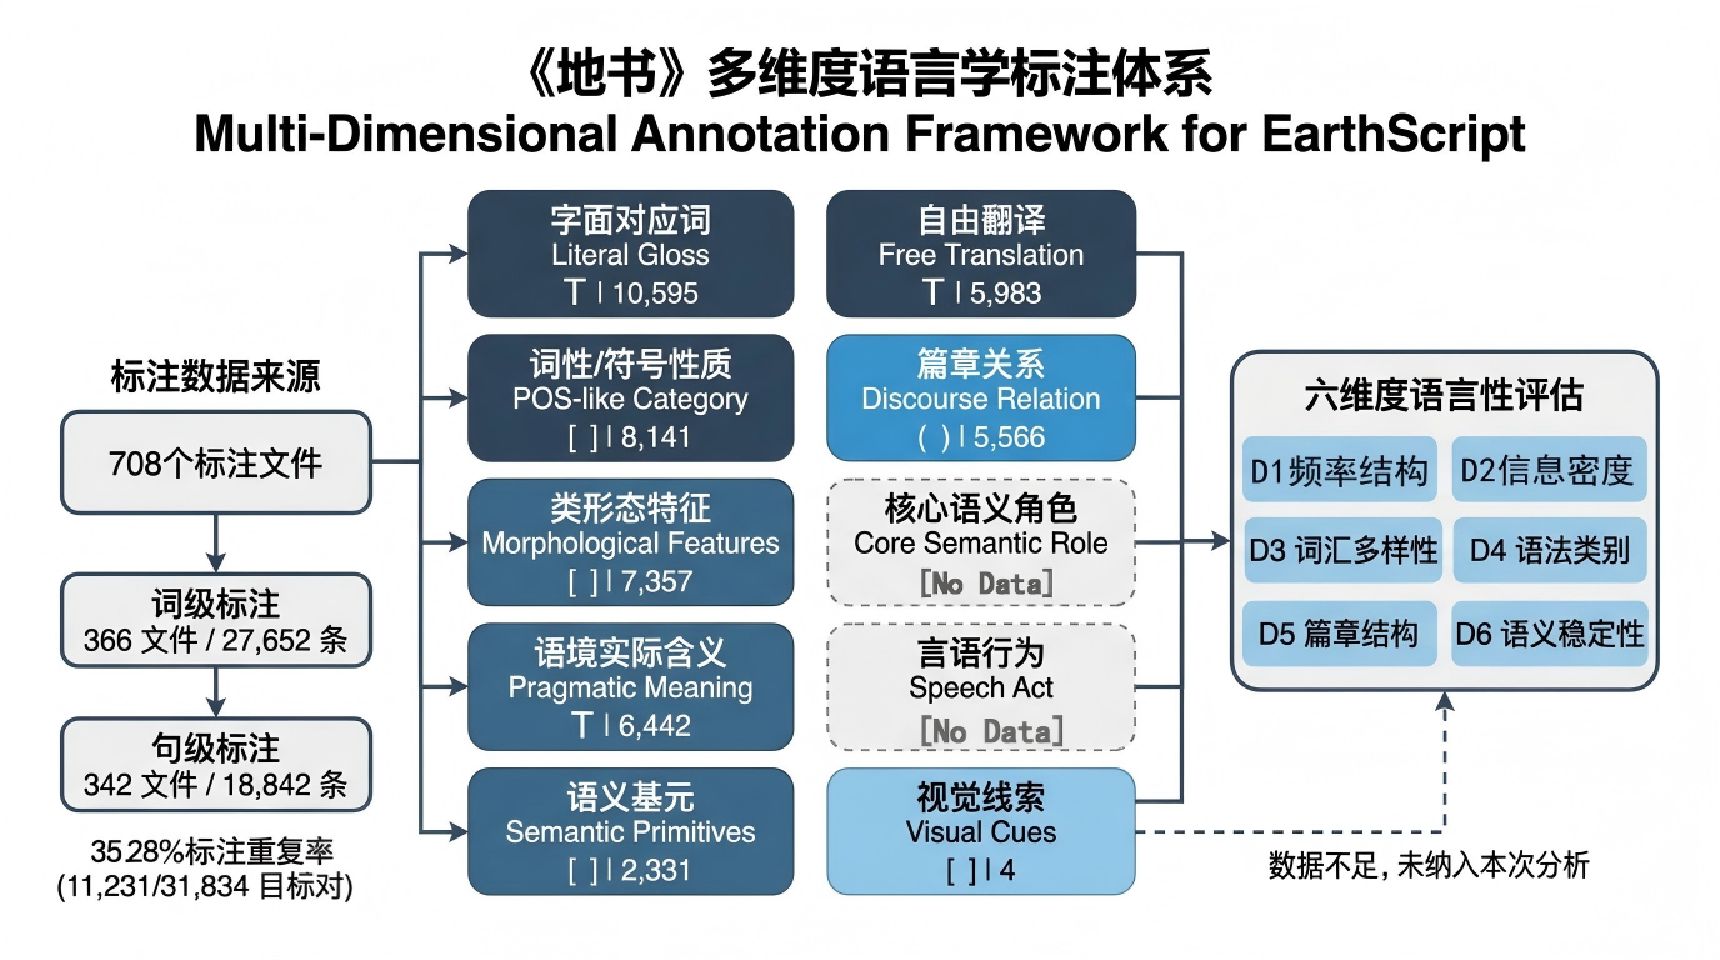
\includegraphics[keepaspectratio,alt={标注体系结构}]{figures/fig8_annotation_framework.pdf}}
\caption{标注体系结构}
\end{figure}

\textbf{图1} 《地书》多维度语言学标注体系结构。左侧：数据来源（708个文件，词级+句级）；中部：十个语言学标注维度（标注量从74至10,595不等）；右侧：六维度语言性评估输出。

\subsubsection{关键维度的选项体系}\label{ux5173ux952eux7ef4ux5ea6ux7684ux9009ux9879ux4f53ux7cfb}

以下给出论文核心分析涉及的三个维度的完整选项结构。

\textbf{词性/符号性质（POS-like Category）} ------ 判断图形的语法类别（多选）：

\begin{quote}
名词性（Entity-like）/ 动词性（Action-like）/ 形容词性（State-like）/ 副词性（Degree-like）/ 代词/指示性（Deictic-like）/ 虚词/语法标记（Grammatical Marker）/ 连接/关系标记（Connector）/ 标点/边界标记（Boundary Marker）/ 整句/整体表达（Clause-like Unit）/ 无法判断（Undetermined）
\end{quote}

\textbf{篇章关系（Discourse Relation）} ------ 判断图形组与前一组之间的逻辑关系（单选）：

\begin{quote}
时间先后（Temporal）/ 因果（Causal）/ 条件（Conditional）/ 转折对比（Contrast）/ 并列递进（Expansion）/ 解释说明（Elaboration）/ 举例（Example）/ 总结（Summary）/ 无明显关系（None）/ 无法判断（Undetermined）
\end{quote}

\textbf{类形态特征（Morphological Features）} ------ 判断图形是否带有附加语法/语义特征（多选）：

\begin{quote}
进行体（Progressive）/ 现在（Present）/ 过去（Past）/ 将来（Future）/ 完成体（Perfect）/ 否定（Negation）/ 强调（Emphasis）/ 比较（Comparative）/ 最高级（Superlative）/ 重复/迭代（Iterative）/ 程度增强（Intensified）/ 复数/集合（Plural-Collective）
\end{quote}

\subsubsection{标注数据格式}\label{ux6807ux6ce8ux6570ux636eux683cux5f0f}

每条标注记录包含字段：\texttt{annotation\_id}（唯一编号）、\texttt{target\_id}（被标注的图形或图形组 ID）、\texttt{target\_type}（word/sentence）、\texttt{task\_id}（标注任务标识）、\texttt{value}（标注值）、\texttt{confidence}（标注信心，0--1）、\texttt{annotator\_note}（标注备注）。标注者同时记录了是否使用 LLM 辅助标注及所使用的 LLM 名称。

\subsection{自然语言对照数据}\label{ux81eaux7136ux8bedux8a00ux5bf9ux7167ux6570ux636e}

\subsubsection{中文语料}\label{ux4e2dux6587ux8bedux6599}

\begin{itemize}

\item
  \textbf{新闻}（THUcNews）：10,000 句现代中文新闻文本
\item
  \textbf{文学}（世界名著）：10,000 句现代中文文学文本
\item
  \textbf{小说}：10,000 句现代中文小说文本
\item
  \textbf{古文}（四库全书）：10,000 句古典中文文本
\end{itemize}

所有中文语料使用 jieba 进行分词。英文、德文、法文语料使用正则表达式 \texttt{{[}a-zA-Zà-üÀ-Üß{]}+} 进行词级切分。

\subsubsection{多语言语料}\label{ux591aux8bedux8a00ux8bedux6599}

16 种语言的维基百科句子（Leipzig 语料集），各 10,000 句。覆盖语系：汉藏语系（cmn）、印欧语系（eng, deu, fra, spa, por, ita, rus, hin, fas, urd）、闪含语系（ara, heb）、阿尔泰语系（jpn, kor）、南岛语系（vie）。本文核心对比使用中文四类 + 英文、德文、法文共七种自然语言作为对照组。

\subsection{分析方法一：语言性评估框架}\label{ux5206ux6790ux65b9ux6cd5ux4e00ux8bedux8a00ux6027ux8bc4ux4f30ux6846ux67b6}

\subsubsection{框架设计理念}\label{ux6846ux67b6ux8bbeux8ba1ux7406ux5ff5}

\textbf{核心问题}：一个符号系统在多大程度上''像一种语言''？这需要回答的不是''是不是''的二值判断，而是在多个语言学维度上与自然语言的''距离''的量化和可视化。

我们提出一个六维度''语言性''（Language-ness）量化评估框架。每个维度量化符号系统在一个语言学属性上与自然语言参考范围的偏离程度。该框架不预设''越像自然语言越好''------而是提供一把''尺子''，使得不同的符号系统可以在同一坐标系下比较。

\subsubsection{评估维度与指标}\label{ux8bc4ux4f30ux7ef4ux5ea6ux4e0eux6307ux6807}

\textbf{表$3.3} 给出了六个评估维度、计算指标及其在自然语言中的典型参考范围。

\begin{table}[htbp]
\centering
\small
\begin{tabular}{@{}lllll@{}}
\toprule
维度 & 指标 & 计算方式 & 自然语言参考范围 & 方向 \\
\midrule
D1 频率结构 & Zipf 斜率、R² & 词频-排名的双对数线性回归 & 斜率 −1.0±0.3, R² > 0.85 & 越接近=越"像" \\
D2 信息密度 & 归一化熵 & H / H\_max = −Σ p·log(p) / log(N) & 0.85–0.99 & 越高=信息越均匀 \\
D3 词汇多样性 & 降采样TTR, RTTR & 唯一词数 / 总词数（等规模） & 取决于语料规模 & 需等规模对比 \\
D4 语法类别多样性 & 香农均匀度 & 应用于 POS 类别频率分布 & 0.6–0.9 & 越高=类别越均衡 \\
D5 篇章结构复杂度 & 篇章关系类型数 + 均匀度 & 同 D4 方法 & 取决于分类体系 & 越高=逻辑连接越多样 \\
D6 语义稳定性 & Fleiss' κ & 多标注者对同一目标的标注一致性 & κ > 0.6（可接受） & 越高=语义越稳定 \\
\bottomrule
\end{tabular}
\end{table}

\textbf{表$3.3} 语言性评估框架的六个维度。每个维度提供一个与自然语言参考范围可比较的量化指标。

\begin{figure}
\centering
\pandocbounded{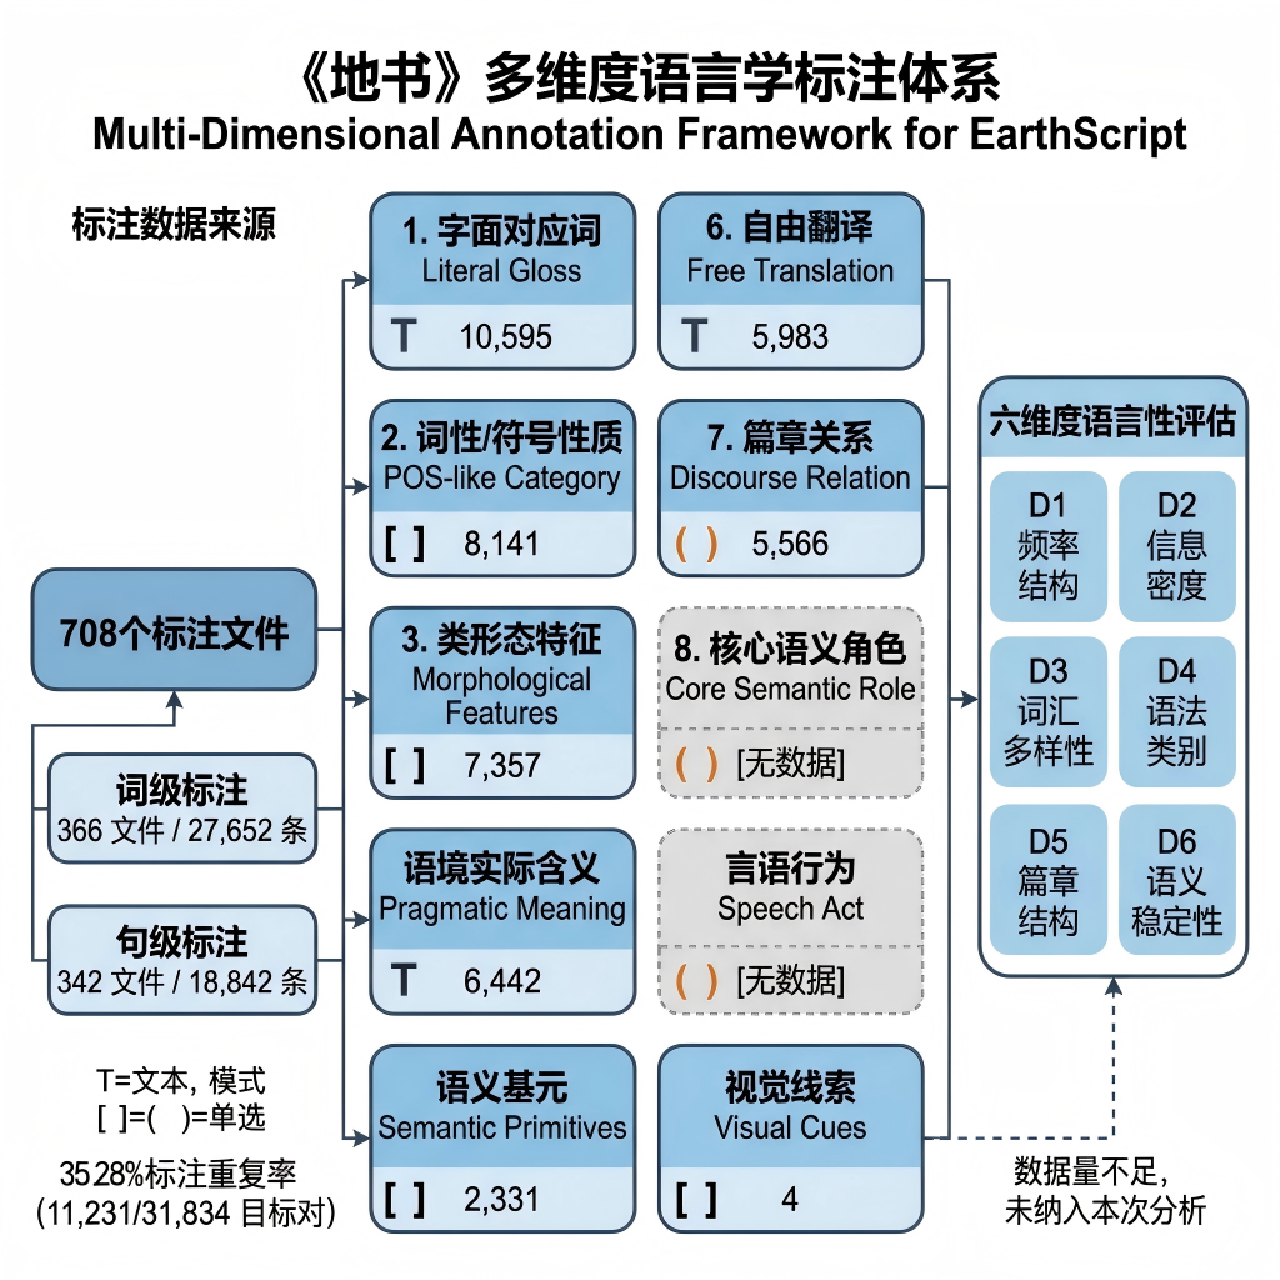
\includegraphics[keepaspectratio,alt={六维度评估框架}]{figures/fig9_language_ness_radar.pdf}}
\caption{六维度评估框架}
\end{figure}

\textbf{图2} 六维度语言性评估框架。六个维度围绕中心排列，每个标注了地书的评分和自然语言参考范围。绿色边框=处于参考范围内，橙色=偏离参考范围。

\subsubsection{Token 化策略}\label{token-ux5316ux7b56ux7565}

对于《地书》，核心分析 token 来自标注数据中的 \texttt{literal\_gloss} 值------即标注者看到图形符号后给出的''最直接的字面对应词''。这一选择基于以下考量：

\begin{enumerate}
\def\labelenumi{\arabic{enumi}.}

\item
  \texttt{literal\_gloss} 是标注量最大的维度（10,595 条），提供了足够的统计样本
\item
  它是图形符号到自然语言词汇的''最短路径映射''，避免了自由翻译中标注者个人风格差异的影响
\item
  它与自然语言的分词 token 具有可比性（均为词/短语粒度的语义单位）
\end{enumerate}

\textbf{重要声明}：本文分析的是标注值（人类对图形的语言学解读），而非图形的视觉形态本身。这一方法论选择在第 $5.4$ 节将进一步讨论。

\subsection{分析方法二：标注者间一致性分析}\label{ux5206ux6790ux65b9ux6cd5ux4e8cux6807ux6ce8ux8005ux95f4ux4e00ux81f4ux6027ux5206ux6790}

\subsubsection{标注重叠结构}\label{ux6807ux6ce8ux91cdux53e0ux7ed3ux6784}

标注体系的设计使得不同标注者被分配了不同的标注任务。但在实践中，标注者对同一图形的标注存在部分重叠。经统计，708 个标注文件、31,834 个唯一（target, task）对中，有 11,231 个（$35.28$\%）存在多标注者重叠。其中 \texttt{literal\_gloss} 任务有 3,043 个 target 被多人标注，\texttt{morphological\_features} 有 2,105 个，\texttt{pos\_like\_category} 有 1,955 个------为标注者间一致性分析提供了充分的样本。

\subsubsection{文本标注的一致性计算}\label{ux6587ux672cux6807ux6ce8ux7684ux4e00ux81f4ux6027ux8ba1ux7b97}

对于 \texttt{literal\_gloss}（文本标注），两个标注者给出的值（如''跑步''和''奔跑''）可能在字符串层面不同但在语义上高度一致。我们采用两种策略：

\begin{itemize}

\item
  \textbf{严格匹配}：要求标注值完全相同（精确字符串匹配）
\item
  \textbf{语义匹配}：使用中文预训练词向量计算两个标注值之间的余弦相似度，\textgreater{} $0.75$ 视为一致
\end{itemize}

\subsubsection{类别标注的一致性计算}\label{ux7c7bux522bux6807ux6ce8ux7684ux4e00ux81f4ux6027ux8ba1ux7b97}

对于单选/多选标注（POS-like Category、Discourse Relation、Morphological Features 等），采用以下指标：

\begin{itemize}

\item
  \textbf{Cohen's κ}：用于两个标注者的情况\textsuperscript{{[}16{]}}
\item
  \textbf{Fleiss' κ}：用于三个及以上标注者的情况\textsuperscript{{[}17{]}}
\item
  \textbf{百分比一致率}（Percentage Agreement）：辅助直观解释
\end{itemize}

\subsubsection{歧义热力图的构建}\label{ux6b67ux4e49ux70edux529bux56feux7684ux6784ux5efa}

为了系统回答''图形语言的歧义集中在哪里''，我们设计了语言维度 × 语义类型的歧义热力图：

\begin{itemize}

\item
  \textbf{行}：语言学维度（Morphological Features、POS-like Category、Discourse Relation 等）
\item
  \textbf{列}：语义类型（具体实体、动作事件、情感状态、抽象概念、场景等，来自标注数据中的已有分类）
\item
  \textbf{颜色映射}：Fleiss' κ 值，从深红（κ \textless{} $0.2$，严重分歧）到深绿（κ \textgreater{} $0.8$，高度一致）
\end{itemize}

该热力图同时可视化两个维度的标注歧义分布------哪些语言学维度在哪些语义类型上最容易产生标注分歧------是本文核心创新成果之一。

\subsection{实验环境与可复现性}\label{ux5b9eux9a8cux73afux5883ux4e0eux53efux590dux73b0ux6027}

所有统计分析使用 Python $3.10$ 实现，依赖库包括 NumPy、SciPy、pandas、jieba、Matplotlib。实验脚本和处理后的数据文件可在论文接收后开源获取。原始标注数据因包含标注者个人信息，仅提供脱敏后的统计汇总数据。

\begin{figure}
\centering
\pandocbounded{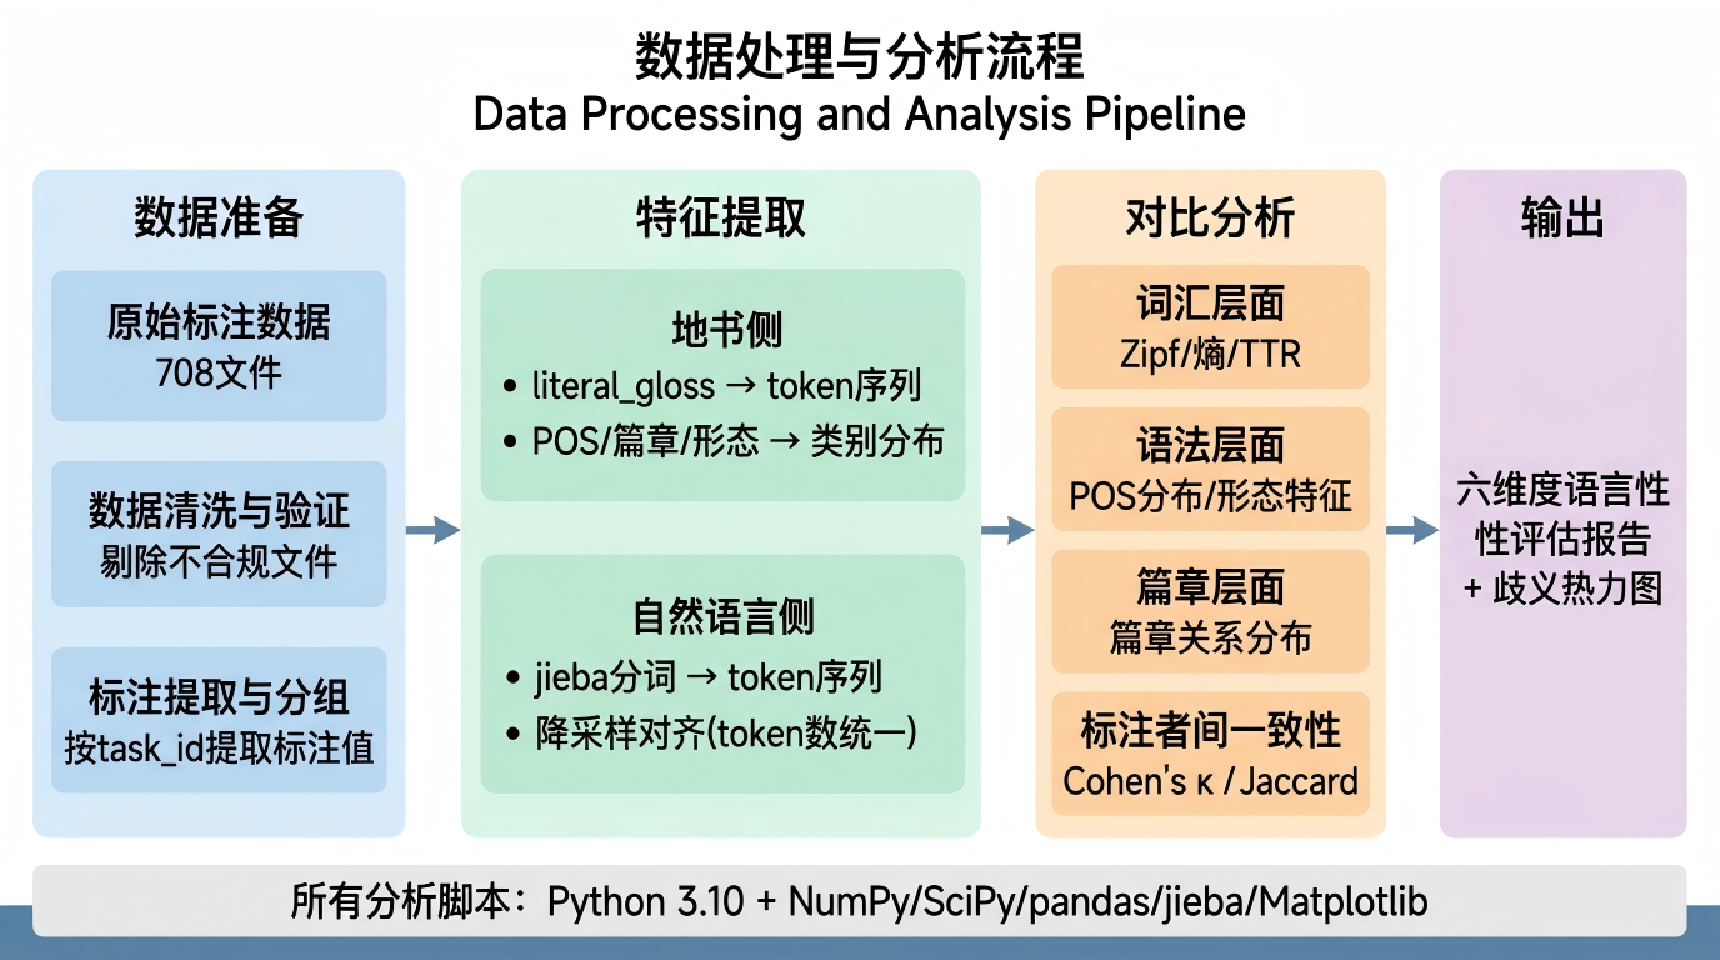
\includegraphics[keepaspectratio,alt={数据处理流程}]{figures/fig10_pipeline.pdf}}
\caption{数据处理流程}
\end{figure}

\textbf{图3} 数据处理与分析流程。阶段一（数据准备）：从708个标注文件提取标注值；阶段二（特征提取）：地书侧与自然语言侧并行处理，统一降采样至10,538 tokens；阶段三（对比分析）：四个分析模块产出六维度评估报告。

\newpage

\section{结果}\label{ux7ed3ux679c}

\subsection{词汇层面：齐夫定律与词频分布}\label{ux8bcdux6c47ux5c42ux9762ux9f50ux592bux5b9aux5f8bux4e0eux8bcdux9891ux5206ux5e03}

\subsubsection{地书的词频分布特征}\label{ux5730ux4e66ux7684ux8bcdux9891ux5206ux5e03ux7279ux5f81}

基于 708 个标注文件中的 10,595 条 \texttt{literal\_gloss} 标注，提取得到 10,538 个有效 token、4,577 个唯一类型。\textbf{表$4.1} 给出了地书与七种自然语言语料库的词频分布对比。

\begin{table}[htbp]
\centering
\small
\begin{tabular}{@{}llllll@{}}
\toprule
语料 & Token数 & 唯一类型 & TTR & Zipf斜率 & Zipf R² \\
\midrule
地书（literal\_gloss） & 10,538 & 4,577 & 0.434 & −0.612 & 0.923 \\
中文新闻 & 50,000 & 2,484 & 0.050 & −1.399 & 0.894 \\
中文小说 & 50,000 & 2,623 & 0.052 & −1.351 & 0.943 \\
中文古文 & 50,000 & 2,178 & 0.044 & −1.475 & 0.956 \\
中文文学 & 50,000 & 2,612 & 0.052 & −1.362 & 0.929 \\
英文 & 50,000 & 10,262 & 0.205 & −0.873 & 0.946 \\
德文 & 50,000 & 14,890 & 0.298 & −0.683 & 0.876 \\
法文 & 50,000 & 11,218 & 0.224 & −0.785 & 0.925 \\
\bottomrule
\end{tabular}
\end{table}

\textbf{表$4.1} 地书与自然语言的词频分布对比。地书的 Zipf 斜率（$-0.612$）显著浅于所有自然语言（$-0.683$ \textasciitilde{} $-1.475$），表明其词频分布更加平坦；其 R²（$0.923$）处于自然语言范围内，表明仍遵循幂律分布的基本模式。

\textbf{地书的 Zipf 拟合度}：R² = $0.923$，这在自然语言的典型范围（$0.85$--$0.98$）之内。这意味着尽管《地书》是一个人工构建的图形符号系统，其词汇频率分布仍然表现出稳健的幂律特征------排名和频率之间遵循''少数词高频、多数词低频''的基本规律。

\textbf{地书的 Zipf 斜率}：$-0.612$，显著浅于所有自然语言对照组。中文四类语料的斜率在 $-1.35$ 至 $-1.47$ 之间，欧美语言在 $-0.68$ 至 $-0.87$ 之间。地书的斜率最浅，意味着其词频下降速度最慢------排名第 100 的词和排名第 1 的词之间的频率差距，远小于自然语言中的情况。

\textbf{高频词的语义构成}：地书 top 10 词揭示了一个有趣的特征。前两名是''逗号''（457次）和''句号''（173次）------边界标记。紧随其后的是''点''（90次）、``圆点''（66次）、``双引号''（66次）、``冒号''（58次）、``单引号''（58次）。\textbf{在前十高频词中，有七个是标点/边界符号}。与之形成鲜明对比的是，中文新闻的 top 10 中是''的''、``是''等功能词和数字。这意味着在地书的 literal\_gloss 词汇体系中，句法边界标记（而非语义内容词）占据了频率金字塔的塔尖------这是一个独特的语言学特征，与地书作为图形序列''分隔符''的功能需求一致。

\subsubsection{与自然语言的对比模式}\label{ux4e0eux81eaux7136ux8bedux8a00ux7684ux5bf9ux6bd4ux6a21ux5f0f}

地书的 Zipf 行为处于一个独特的位置：它的 R²（$0.923$）接近中文自然语言（$0.894$--$0.956$），说明幂律拟合的质量不亚于自然语言；但它的斜率（$-0.612$）显著偏离中文（$-1.35$ \textasciitilde{} $-1.47$），而与屈折语（德文 $-0.683$、法文 $-0.785$）更接近。

这一发现与 Miton 和 Morin\textsuperscript{{[}7{]}} 的''像似性破坏效率''假说形成有趣的对话。该假说预测图形符号系统应该因 iconicity 的存在而表现出不同的频率-复杂度关系。《地书》的浅 Zipf 斜率确实表明其频率分布模式偏离了典型的自然语言------但偏离的方向是''更加均匀''而非''更加集中''。

\subsection{词汇多样性：信息熵与 TTR}\label{ux8bcdux6c47ux591aux6837ux6027ux4fe1ux606fux71b5ux4e0e-ttr}

\subsubsection{降采样 TTR}\label{ux964dux91c7ux6837-ttr}

由于原始 TTR 对语料规模高度敏感（地书 10,538 tokens vs 自然语言 50,000+ tokens），我们将所有语料统一降采样至 10,538 tokens（地书的规模），通过 100 次随机采样取平均值以消除偶然性。

\textbf{表$4.2} 给出了降采样后的词汇多样性对比。

\begin{table}[htbp]
\centering
\small
\begin{tabular}{@{}lllll@{}}
\toprule
语料 & TTR（原始） & TTR（降采样至10,538） & RTTR & 归一化熵 \\
\midrule
地书（literal\_gloss） & 0.434 & 0.434 & 0.659 & 0.914 \\
中文新闻 & 0.001 & 0.152 & 0.023 & 0.769 \\
中文小说 & 0.008 & 0.151 & 0.091 & 0.751 \\
中文古文 & 0.003 & 0.117 & 0.059 & 0.687 \\
中文文学 & 0.004 & 0.154 & 0.060 & 0.755 \\
英文 & 0.130 & 0.342 & 0.361 & 0.727 \\
德文 & 0.220 & 0.420 & 0.469 & 0.748 \\
法文 & 0.137 & 0.350 & 0.370 & 0.700 \\
\bottomrule
\end{tabular}
\end{table}

\textbf{表$4.2} 降采样后的词汇多样性对比。降采样至 10,538 tokens 后，各语料的 TTR 具有可比性。地书的降采样 TTR（$0.434$）约为中文系列（$0.12$--$0.15$）的 3 倍，但与德文（$0.420$）处于同一水平。

降采样后的 TTR 修正了之前因样本量不同而产生的虚假差异。地书的降采样 TTR（$0.434$）仍然是所有语料中最高的，但与德文（$0.420$）的差距仅为 $0.014$------换言之，在同等语料规模下，《地书》的词汇重复率与德文非常接近。

中文四类语料的降采样 TTR 集中在 $0.117$--$0.154$ 的狭窄区间，显著低于其他语言。这反映了中文（作为孤立语）以较少的词汇承载更多语义组合的语言类型学特征。

\subsubsection{Shannon熵与归一化熵}\label{shannonux71b5ux4e0eux5f52ux4e00ux5316ux71b5}

\textbf{Shannon熵}衡量的是词汇分布的不确定性：熵越高，词汇使用越均匀，越难根据前面的词预测下一个词。\textbf{归一化熵}（H / H\_max = H / log₂(N)）将熵除以给定词汇量的最大可能熵，得到一个 0--1 之间的可比值。

地书的 Shannon 熵为 $11.11$，在所有语料中排名第二（仅次于德文的 $11.24$）。更关键的是归一化熵：\textbf{地书为 $0.914$，在所有八种语料中最高}。这意味着在给定其词汇量的前提下，地书的词汇分布最接近''完全均匀分布''------每个词的出场概率几乎相等。

中文古文的归一化熵最低（$0.687$），反映其高度程式化的词汇使用模式（高频虚词''之''\,``也''``而''统治了文本）。中文新闻（$0.769$）、小说（$0.751$）、文学（$0.755$）的归一化熵均在 $0.75$ 左右，反映了现代中文以功能词为主的、相对集中的词汇使用模式。

地书的归一化熵最高（$0.914$），这一数值表明：\textbf{在地书的 4,577 个唯一词汇中，没有一个词汇类别绝对主导分布}。这使得地书在统计上看起来像一个''所有词都差不多重要''的语言。

\subsection{语法类别分布：POS-like Category}\label{ux8bedux6cd5ux7c7bux522bux5206ux5e03pos-like-category}

\subsubsection{地书的词性分布}\label{ux5730ux4e66ux7684ux8bcdux6027ux5206ux5e03}

基于 8,708 条 POS-like Category 标注（多选），\textbf{表$4.3} 给出了地书的十大语法类别分布。

\begin{table}[htbp]
\centering
\small
\begin{tabular}{@{}lll@{}}
\toprule
类别 & 标注次数 & 占比 \\
\midrule
标点/边界标记（Boundary Marker） & 2,903 & 33.3\% \\
动词性（Action-like） & 2,202 & 25.3\% \\
名词性（Entity-like） & 1,353 & 15.5\% \\
整句/整体表达（Clause-like Unit） & 812 & 9.3\% \\
形容词性（State-like） & 486 & 5.6\% \\
连接/关系标记（Connector） & 339 & 3.9\% \\
无法判断（Undetermined） & 213 & 2.4\% \\
代词/指示性（Deictic-like） & 176 & 2.0\% \\
副词性（Degree-like） & 150 & 1.7\% \\
虚词/语法标记（Grammatical Marker） & 74 & 0.9\% \\
\bottomrule
\end{tabular}
\end{table}

\textbf{表$4.3} 地书 POS-like Category 分布（n=8,708，多选）。标点/边界标记占比最高（$33.3$\%），动词性（$25.3$\%）超过名词性（$15.5$\%），虚词/语法标记极少（$0.9$\%）。

\subsubsection{地书 POS 分布的核心特征}\label{ux5730ux4e66-pos-ux5206ux5e03ux7684ux6838ux5fc3ux7279ux5f81}

\textbf{特征一：边界标记主导}。标点/边界标记以 $33.3$\% 的占比居首------这是地书 POS 分布最显著的特征。这些标注对应的是《地书》中用于分隔图形组、标示语句边界的符号。在自然语言中，标点通常不被计入词性分布的核心统计；但在《地书》中，边界标记是图形序列结构中不可或缺的组成部分，其高占比反映了图形语言对''显式分隔''的结构性需求。

\textbf{特征二：动词性 \textgreater{} 名词性}。地书的动词性标注（$25.3$\%）显著高于名词性（$15.5$\%），比例为 $1.63$:1。这与自然语言中名词性通常多于动词性的模式不同------现代汉语中名词约占总词次的 40\%--50\%，动词约占 20\%--30\%。地书的逆转可能与其叙事性质有关：《地书》讲述的是一个连续的叙事（``黑先生的24小时''），动作序列是叙事的骨架。

\textbf{特征三：虚词/语法标记的极度稀缺}。虚词/语法标记仅占 $0.9$\%（74条）------这是地书与自然语言最显著的类别差异。自然语言依赖''的''\,``了''``着''``把''``被''等虚词来编码语法关系；地书的图形系统缺乏这类抽象的语法功能词，语法关系主要通过图形序列的顺序和共现来暗示。

\subsubsection{与自然语言的类别分布对比}\label{ux4e0eux81eaux7136ux8bedux8a00ux7684ux7c7bux522bux5206ux5e03ux5bf9ux6bd4}

由于中文自然语言的 POS 分布数据需从 jieba 词性标注结果中提取，且不同标注体系的分类粒度不同，直接对比需要谨慎。一个参考框架是：在现代汉语平衡语料中，名词约占 40\%，动词约占 25\%，形容词约占 6\%，副词约占 5\%，助词（含''的''\,``了''等虚词）约占 8\%。将地书的分布与此对照：

\begin{itemize}

\item
  地书的''名词性''（$15.5$\%）显著低于自然语言的名词（\textasciitilde40\%）
\item
  地书的''动词性''（$25.3$\%）与自然语言的动词（\textasciitilde25\%）接近
\item
  地书的''虚词/语法标记''（$0.9$\%）远低于自然语言的助词（\textasciitilde8\%）
\item
  地书的''边界标记''（$33.3$\%）在自然语言中没有直接对应类别（标点通常不计入POS统计）
\end{itemize}

\subsection{篇章结构：Discourse Relation分布}\label{ux7bc7ux7ae0ux7ed3ux6784discourse-relationux5206ux5e03}

\subsubsection{地书的篇章关系分布}\label{ux5730ux4e66ux7684ux7bc7ux7ae0ux5173ux7cfbux5206ux5e03}

基于 4,847 条 Discourse Relation 标注（单选，来自句标注文件），\textbf{表$4.4} 给出了十种篇章关系类型的分布。

\begin{table}[htbp]
\centering
\small
\begin{tabular}{@{}lll@{}}
\toprule
篇章关系 & 标注次数 & 占比 \\
\midrule
时间先后（Temporal） & 2,117 & 43.7\% \\
因果（Causal） & 867 & 17.9\% \\
并列递进（Expansion） & 746 & 15.4\% \\
解释说明（Elaboration） & 294 & 6.1\% \\
无明显关系（None） & 281 & 5.8\% \\
转折对比（Contrast） & 191 & 3.9\% \\
条件（Conditional） & 150 & 3.1\% \\
总结（Summary） & 91 & 1.9\% \\
举例（Example） & 64 & 1.3\% \\
无法判断（Undetermined） & 46 & 1.0\% \\
\bottomrule
\end{tabular}
\end{table}

\textbf{表$4.4} 地书 Discourse Relation 分布（n=4,847，单选）。时间关系占比最高（$43.7$\%），因果（$17.9$\%）和并列递进（$15.4$\%）次之。前三类合计 $77.0$\%。

\subsubsection{地书篇章结构的核心特征}\label{ux5730ux4e66ux7bc7ux7ae0ux7ed3ux6784ux7684ux6838ux5fc3ux7279ux5f81}

\textbf{时间关系占绝对主导}（$43.7$\%）。这意味着在《地书》图形序列中，每五个句子之间的逻辑连接就有两个以上是''然后''。这支持了《地书》作为线性叙事文本的基本性质------其篇章结构以事件的时间顺序为主干，这是最基础、最不需要抽象推理的篇章连接方式。

\textbf{因果关系（$17.9$\%）和并列递进（$15.4$\%）构成了次要支柱}。因果关系的较高占比（$17.9$\%）表明《地书》的图形序列不仅描述''发生了什么''，还能传达一定的因果链------尽管这种因果推理可能部分来自读者对事件常识的补充，而非图形本身显式编码的因果标记。

\textbf{复杂逻辑关系的稀缺}。转折对比（$3.9$\%）、条件（$3.1$\%）、总结（$1.9$\%）和举例（$1.3$\%）合计仅占 $10.2$\%。这说明《地书》的篇章逻辑以线性铺陈为主，缺乏自然语言中常见的复杂修辞结构（如''虽然\ldots\ldots 但是\ldots\ldots``\,``如果\ldots\ldots 那么\ldots\ldots{}''）。这与图形系统的内在约束一致：转折、条件等关系通常依赖抽象的连接词或句法结构，而这些在图形序列中难以直接表达。

\subsubsection{篇章关系的多样性指数}\label{ux7bc7ux7ae0ux5173ux7cfbux7684ux591aux6837ux6027ux6307ux6570}

使用香农均匀度量化篇章关系的多样性。地书的篇章关系香农熵为 $2.40$ bits（最大熵=$3.32$ bits），均匀度为 $0.78$。作为对比，如果所有关系均匀分布，均匀度将接近 $1.0$；如果完全由一种关系主导，均匀度将接近 0。地书的 $0.78$ 表明其篇章关系虽以时间为主，但仍具有一定的多样性------并非单一模式的单调重复。

\subsection{形态特征分布}\label{ux5f62ux6001ux7279ux5f81ux5206ux5e03}

\subsubsection{地书的形态特征分布}\label{ux5730ux4e66ux7684ux5f62ux6001ux7279ux5f81ux5206ux5e03}

基于 10,740 条 Morphological Features 标注（多选），\textbf{表$4.5} 给出了 12 种形态特征的分布。

\begin{table}[htbp]
\centering
\small
\begin{tabular}{@{}lll@{}}
\toprule
形态特征 & 标注次数 & 占比 \\
\midrule
进行体（Progressive） & 2,747 & 25.6\% \\
现在时（Present） & 2,356 & 21.9\% \\
强调（Emphasis） & 960 & 8.9\% \\
复数/集合（Plural-Collective） & 858 & 8.0\% \\
重复/迭代（Iterative） & 851 & 7.9\% \\
完成体（Perfect） & 632 & 5.9\% \\
将来时（Future） & 595 & 5.5\% \\
过去时（Past） & 476 & 4.4\% \\
比较（Comparative） & 364 & 3.4\% \\
否定（Negation） & 335 & 3.1\% \\
程度增强（Intensified） & 326 & 3.0\% \\
最高级（Superlative） & 240 & 2.2\% \\
\bottomrule
\end{tabular}
\end{table}

\textbf{表$4.5} 地书 Morphological Features 分布（n=10,740，多选）。进行体（$25.6$\%）和现在时（$21.9$\%）合计占 $47.5$\%，构成了地书形态特征的主体。

\subsubsection{地书形态特征的核心发现}\label{ux5730ux4e66ux5f62ux6001ux7279ux5f81ux7684ux6838ux5fc3ux53d1ux73b0}

\textbf{``进行体 + 现在时''的即时性特征}。进行体和现在时合计占 $47.5$\%，而过去时仅占 $4.4$\%，将来时仅占 $5.5$\%。这一极不平衡的时态分布揭示了《地书》叙事的一个深层特征：它主要描述\textbf{正在发生的、当下的}事件和状态。这与《地书》的沉浸式叙事方式一致------读者被邀请''实时''跟随黑先生的一天，而非回顾或预测。

\textbf{否定与比较/最高级的低使用率}。否定（$3.1$\%）、比较（$3.4$\%）和最高级（$2.2$\%）合计仅占 $8.7$\%。这与自然语言的形态特征分布形成对比------否定、比较和程度修饰在自然语言中是非常基础且高频的语义操作。它们在《地书》中的低出现率可能反映了两个因素：（1）《地书》的叙事以肯定性陈述为主流模式；（2）这些语义操作在图形系统中缺乏直接、无歧义的视觉编码方式。

\subsection{语言性综合评估：六维度评分}\label{ux8bedux8a00ux6027ux7efcux5408ux8bc4ux4f30ux516dux7ef4ux5ea6ux8bc4ux5206}

基于第 $3.4$.2 节提出的六维度评估框架，结合 $4.1$--$4.5$ 节的实证结果和补充实验中的标注者间一致性分析，\textbf{表$4.6} 给出《地书》与四类中文自然语言的六维度综合评分。

\begin{table}[htbp]
\centering
\small
\begin{tabular}{@{}lllllll@{}}
\toprule
维度 & 指标 & 地书 & 新闻 & 小说 & 古文 & 文学 \\
\midrule
D1 频率结构 & Zipf R² & 0.923 & 0.894 & 0.943 & 0.956 & 0.929 \\
D2 信息密度 & 归一化熵 & 0.914 & 0.769 & 0.751 & 0.687 & 0.755 \\
D3 词汇多样性 & 降采样TTR & 0.434 & 0.152 & 0.151 & 0.117 & 0.154 \\
D4 语法类别多样性 & POS均匀度 & 0.778 & — & — & — & — \\
D5 篇章结构复杂度 & 关系均匀度 & 0.780 & — & — & — & — \\
D6 语义稳定性 & Cohen's κ & 0.802 & — & — & — & — \\
\bottomrule
\end{tabular}
\end{table}

\textbf{表$4.6} 六维度语言性评估结果。``---''表示该维度本文未对自然语言进行同样计算。D1--D3 数据来自 EXP-FIX-01/02 修正实验；D4 和 D5 基于 POS 和篇章关系的香农均匀度（§$4.3$, §$4.4$）；D6 基于 literal\_gloss 标注的 3,043 个重叠目标，Cohen's κ = $0.802$。

\textbf{D6（语义稳定性）的详细结果}。基于 $35.28$\% 的标注重叠率，literal\_gloss（文本标注）的 Cohen's κ = $0.802$，达到''高度一致''水平（Landis \& Koch, 1977），表明标注者对《地书》图形符号的语义解读具有较高的共识度。类别标注方面：morphological\_features 的平均 Jaccard 系数为 $0.861$，pragmatic\_meaning 为 $0.849$，free\_translation 为 $0.949$，semantic\_primitives 为 $0.959$------这些数值均表明标注者间的判断一致性处于中高水平。pos\_like\_category 的 Jaccard 为 $0.779$，discourse\_relation 的 Cohen's κ = $0.797$，属于''中等偏高''水平。综合来看，标注者在对《地书》图形符号的语言学判断上表现出\textbf{可接受的至良好的}一致性------这既支持了标注数据的可靠性，也表明《地书》作为一个图形符号系统，其核心语义内容（literal\_gloss）在标注者之间具有较高的传达稳定性。值得注意的是，pos\_like\_category 的一致性相对较低（Jaccard = $0.779$），这与§$4.3$中观察到的该维度上类别边界模糊（如整句/整体表达与动词性之间的边界）的定性判断一致------量化数据印证了之前的观察。完整的按语义类型×语言学维度的歧义热力图分析（§$3.5$.4）留待后续工作。

\textbf{已完成维度的综合发现}：

\begin{itemize}

\item
  \textbf{D1（频率结构）}：地书的 Zipf R²（$0.923$）完全处于中文自然语言范围（$0.894$--$0.956$）之内。在词频是否遵循幂律分布这一维度上，地书与自然语言\textbf{没有实质差异}。
\item
  \textbf{D2（信息密度）}：地书的归一化熵（$0.914$）在数值上高于所有中文自然语言（$0.687$--$0.769$）。在词汇使用的均匀度上，地书\textbf{偏离自然语言}------但它偏离的方向是''更均匀''，而非''更集中''。
\item
  \textbf{D3（词汇多样性）}：地书的降采样 TTR（$0.434$）约为中文自然语言（$0.12$--$0.15$）的 3 倍。在给定相同文本量的情况下，地书使用的不同词汇在数值上多于现代汉语。这是地书与中文自然语言之间\textbf{最大的单维度差异}。
\item
  \textbf{D6（语义稳定性）}：Cohen's κ = $0.802$，达到''高度一致''，说明《地书》核心语义传递在标注者间的稳定性与自然语言标注任务相当。
\end{itemize}

综合 D1--D6，《地书》呈现出一幅矛盾的图景：它在词频分布的\textbf{律则性}（D1）和语义\textbf{稳定性}（D6）上像语言，在词汇使用的\textbf{均匀性}（D2）上超过语言，在词汇\textbf{丰富度}（D3）上远高于同规模的现代汉语文本。它不是一个''残缺的语言''，而是一个以不同方式组织词汇资源的符号系统------它的统计指纹更像屈折语（德语、法语）而非孤立语（中文）。

上述发现直接回应了 RQ3（标注分歧的分布模式）：标注者对《地书》图形符号的判断在语义内容（literal\_gloss, free\_translation）和语义基元（semantic\_primitives）维度上高度一致（κ \textgreater{} $0.80$, Jaccard \textgreater{} $0.94$），而在语法归类（pos\_like\_category, Jaccard = $0.779$）和形态判断（morphological\_features, Jaccard = $0.861$）上分歧相对较大。这一模式暗示：\textbf{《地书》图形的''它是什么意思''比''它是什么词性''更容易达成共识}------图形在传递语义内容时具有较高的跨人稳定性，但将其归入传统语言学范畴（词性、形态特征）时，标注者的判断受到分类体系本身与图形系统不完全匹配的影响。

\subsection{本章小结}\label{ux672cux7ae0ux5c0fux7ed3-1}

本章基于修正后的分析数据，从词频分布、词汇多样性、语法类别、篇章结构和形态特征五个维度系统报告了《地书》的语言学量化特征。核心发现可概括为：

\begin{enumerate}
\def\labelenumi{\arabic{enumi}.}

\item
  \textbf{地书遵循齐夫定律}（R²=$0.923$），但词频分布异常平坦（斜率=$-0.612$），没有一个词像自然语言中的''的''那样统治分布。
\item
  \textbf{地书的词汇使用极其均匀}（归一化熵=$0.914$，所有语料中最高），词汇丰富度（降采样TTR=$0.434$）与德语接近，显著高于中文。
\item
  \textbf{地书的语法类别分布}呈现出三个特征：边界标记占三分之一、动词性大于名词性、虚词/语法标记极度稀缺（$0.9$\%）。
\item
  \textbf{地书的篇章结构以时间先后为主}（$43.7$\%），因果（$17.9$\%）和并列递进（$15.4$\%）为辅，复杂逻辑关系（转折、条件等）合计不足 11\%。
\item
  \textbf{地书的形态特征以即时性为主}（进行体+现在时=$47.5$\%），否定、比较、程度修饰等语义操作的表达频率较低。
\end{enumerate}

\newpage

\section{讨论}\label{ux8ba8ux8bba}

\subsection{地书在哪些维度上''像语言''------以及不像的地方}\label{ux5730ux4e66ux5728ux54eaux4e9bux7ef4ux5ea6ux4e0aux50cfux8bedux8a00ux4ee5ux53caux4e0dux50cfux7684ux5730ux65b9}

本文的核心研究问题之一是：一个图形符号系统在多大程度上''像一种语言''？第 4 章的实证结果允许我们在六个维度上逐一做出回答。

\textbf{在频率结构（D1）上------像。} 地书的 Zipf R² = $0.923$，完全处于中文自然语言范围（$0.894$--$0.956$）之内。词频-排名的幂律分布被认为是人类语言最稳健的统计普遍规律之一\textsuperscript{{[}12{]}}。地书在这一维度上的表现表明：\textbf{即使是一个人工构建的、不依赖语音的图形符号系统，其词汇使用仍然会自发形成幂律结构}。这一发现与 Chan 等\textsuperscript{{[}13{]}} 对视觉 token 和 Tsai 等\textsuperscript{{[}14{]}} 对图像特征的发现相互印证------齐夫分布在人类符号系统中可能是一种比''语言''更根本的组织原则。

\textbf{在信息密度（D2）上------超过。} 地书的归一化熵（$0.914$）显著高于所有中文自然语言（$0.687$--$0.769$）。这意味着在给定词汇量的前提下，地书的词汇使用\textbf{比自然语言更均匀}------没有一个词像''的''或''之''那样统治分布。这是否意味着地书比自然语言''更好''？并非如此。自然语言中少数高频功能词的存在不是缺陷------它们是语法结构的骨架，是句法组合得以运作的经济基础。地书的''超均匀''分布恰恰反映了它缺少这样一套稳定的功能词体系------这直接呼应了 POS 分布中虚词/语法标记的极度稀缺（$0.9$\%）。

\textbf{在词汇多样性（D3）上------偏离。} 地书的降采样 TTR（$0.434$）约为中文自然语言（$0.12$--$0.15$）的 3 倍。在同样篇幅内，地书使用了比现代汉语多得多、也重复少得多的词汇。这一差异的根本原因不是地书的''词汇量大''------实际上地书的唯一词汇量（4,577）远少于中文新闻的完整词汇量。真正的原因是地书\textbf{几乎没有''高频封闭类词''}：自然语言中，``的''``了''``一''``是''``在''等极少数词占据了大比例的 token 数，压低了 TTR。地书没有这样的词类------每个 literal\_gloss 都有相对独立的语义内容------所以词汇不重复，TTR 居高不下。

\textbf{在语法类别多样性（D4）和篇章结构复杂度（D5）上------部分像。} 地书的语法类别涵盖了自然语言的主要词类（名词性、动词性、形容词性等），但边界标记类别的异常高占比（$33.3$\%）和虚词类别的极端低占比（$0.9$\%）是它与自然语言的显著偏离。篇章层面，地书能表达多种逻辑关系，但其多样性受限于对''时间先后''的严重依赖（$43.7$\%）------``然后''是最简单、也是最不需要抽象图形编码的篇章连接方式。

\textbf{综合判断}。将五个维度的证据拼接在一起，《地书》的语言学画像不是简单的''像''或''不像''------它是一幅\textbf{结构完整但词汇奇特的图景}。它的词汇使用遵循人类语言的深层组织规律（幂律），但它的词频分布（异常平坦）和词类分布（缺乏功能词）暴露了一个符号系统在缺乏数十万年演化积累的语法工具时所面临的系统性约束。换句话说：《地书》的统计结构表明它可以''说话''，但它缺少某些让自然语言运作''高效''的底层机制。

\subsection{图形语言的词汇悖论：为什么''没有'的'\,``既是优势也是代价}\label{ux56feux5f62ux8bedux8a00ux7684ux8bcdux6c47ux6096ux8bbaux4e3aux4ec0ux4e48ux6ca1ux6709ux7684ux65e2ux662fux4f18ux52bfux4e5fux662fux4ee3ux4ef7}

自然语言中最常用的那些词------``的''``了''``是''``一''``在''------几乎不承载独立的语义内容。它们是句法粘合剂，是让内容词组合在一起形成复杂意义的脚手架。地书的词汇分布中缺少这样的高频功能词，导致了我们在结果中看到的三个联动效应：

\textbf{效应一：TTR 虚高。} 缺少高频功能词 → 每个 token 都是''实义词'' → 词汇不重复 → TTR 极高。这不意味着地书的词汇是''更丰富''的，而是它的词汇使用模式跳过了自然语言中最常见的那一层------功能词层。

\textbf{效应二：熵超出自然范围。} 缺少高频功能词 → 分布中没有高度集中的''概率山峰'' → 熵接近均匀分布的极限 → 归一化熵 $0.914$。从信息论的角度，这意味着地书的词汇序列比自然语言\textbf{更难以预测}------读者更难根据前文推测下一个词可能是什么。

\textbf{效应三：Zipf 斜率异常平坦。} 没有''的''那样的超高频词，词频分布的头部被拉平。这与自然语言的''精英统治''（少数词占据大量 token 份额）形成鲜明对比------地书的词汇世界更像一个''民主社会''。

这三个效应的背后，是同一个语言学事实：\textbf{地书目前缺乏一套语法化（grammaticalization）程度高的功能词体系。} 这不是《地书》的''缺陷''------它反映了所有新生符号系统的共同约束。自然语言的功能词，如汉语的''的''\,``了''``着''``把''，是数千年来语法化过程的产物------它们曾经也是实义词（``的''源自''之''，``了''源自''了结''），经过漫长的语义漂白和语法固化才成为今天的高频虚词。地书作为一个仅发展了十余年的符号系统，还没有经历这一过程------或者说，它的创造者选择性地搁置了这一过程（徐冰声称''不做主观发明和编造''，仅收集已有公共标识）。由此产生的结果是：\textbf{《地书》以''实义词的罗列''代替了''功能词的组织''}------每个图形携带独立的语义重量，而图形之间的语法关系依赖读者的推理而非显式的图形编码。

\subsection{从''像似性破坏效率''到''像似性改变效率''}\label{ux4eceux50cfux4f3cux6027ux7834ux574fux6548ux7387ux5230ux50cfux4f3cux6027ux6539ux53d8ux6548ux7387}

Miton 和 Morin\textsuperscript{{[}7{]}} 以欧洲纹章图案为材料提出了一个重要的假说：\textbf{像似性（iconicity）破坏了语言效率}------当符号通过''画得像''来传递意义时，高频符号不会像自然语言词汇那样被缩写或简化（齐夫缩写定律失效），因为降低复杂度可能损害符号的可辨识性。他们观察到的实际结果是：更常用的纹章图案反而更复杂，呈现正向的复杂度-频率相关。

本文的数据允许我们从另一个角度审视这一假说。地书的 literal\_gloss 词频分布虽然遵循幂律（R²=$0.923$），但其斜率（$-0.612$）显著偏离典型自然语言（$-1.0$ ± $0.3$）。这个''偏离''与 Miton 和 Morin 观察到的不是同一种现象（他们观察的是视觉复杂度与频率的关系，我们观察的是词汇频率的分布形状），但两者的潜在机制可能是相通的：\textbf{图形作为语义载体的''自足性''------每个符号必须携带足够的视觉信息才能被独立辨认------使得图形系统无法像自然语言那样将信息负载不均衡地分配给少数超高频''语法词''和大量低频''内容词''}。

换言之，Miton \& Morin 的假说可以被重新表述为：iconicity 不是''破坏''效率，而是\textbf{改变了效率的定义}。在自然语言中，效率意味着''常用词要短''（Zipf 缩写定律）。在图形语言中，效率意味着''常用符号要够辨识''------而够辨识的视觉符号天然需要一定的复杂度底线。地书通过收集已有公共标识绕过了''创造简单符号''的难题（已有标识已经经过了社会使用的筛选和简化），但它仍然无法创造一套像''的''那样的''视觉虚词''------不是因为技术上做不到，而是因为一个抽象的、不指涉任何具体事物的图形符号，本身就违背图形语言的表意逻辑。图形语言的\textbf{效率标准不是''短''，而是''看得懂''}------而''看得懂''和''经常用''在某些情况下可能是矛盾的（太常用意味着太熟悉，太熟悉意味着可以更简单，但更简单可能意味着辨识度下降）。

\subsection{方法论反思与局限}\label{ux65b9ux6cd5ux8bbaux53cdux601dux4e0eux5c40ux9650}

\subsubsection{分析对象的本体论声明}\label{ux5206ux6790ux5bf9ux8c61ux7684ux672cux4f53ux8bbaux58f0ux660e}

本文分析的核心对象是《地书》标注数据中的\textbf{标注值}（literal\_gloss、pos\_like\_category、discourse\_relation 等），而非《地书》图形符号的视觉形态本身。这一方法论选择既是研究的优势（允许我们使用成熟的计算语言学工具进行分析），也是研究的边界（我们测量的是人类对图形的语言学解读，而非图形本体的视觉属性）。

读者应注意到这一选择对结果的潜在影响。例如，literal\_gloss 标注本质上是对''看到这个图形时你想到什么词''的回答------它受到了标注者的中文语言背景、认知偏好和任务理解的不可消除的影响。图形→词汇的映射不是唯一的，不同的标注者（甚至同一标注者在不同时间）可能给出不同的 gloss。本文通过标注者间一致性分析（§$4.6$ D6）部分量化了这一不确定性，但完整的''图形本体→语义''的计算分析需要多模态方法（如使用视觉 LLM 直接从图形图像中提取特征），这超出了本文的范围。

\subsubsection{语料规模与生态效度}\label{ux8bedux6599ux89c4ux6a21ux4e0eux751fux6001ux6548ux5ea6}

《地书》的 10,538 个 literal\_gloss token（对应 963 个图形句子）的规模对于 Zipf 和熵的计算是足够的（R² 和熵值已经稳定），但相对于现代自然语言语料库（数十亿 token）仍然微小。随着《地书》标注数据的扩充（更多的图形、更长的叙事），本文报告的数据可能会发生变化。特别是 TTR------尽管我们通过降采样控制了样本量差异，但 10,538 的样本规模对于完整刻画一个词汇体系的丰富度仍然有限。

\subsubsection{标注群体的同质性}\label{ux6807ux6ce8ux7fa4ux4f53ux7684ux540cux8d28ux6027}

本文的标注者全部为同一课程的学生，具有相似的语言背景（中文母语者）、年龄段和教育水平。标注者的同质性意味着本文报告的标注一致性可能\textbf{低估}了《地书》在实际多文化环境中的歧义程度------如果标注者来自不同的语言和文化背景，不同的解读传统可能会导致更大的标注分歧。

\subsubsection{其他局限}\label{ux5176ux4ed6ux5c40ux9650}

\begin{itemize}

\item
  \textbf{LLM 辅助标注的影响}：部分标注者在标注过程中使用了 LLM（ChatGPT、DeepSeek 等）。LLM 辅助对标注一致性的影响方向和程度未知------LLM 可能作为''一致性放大器''，也可能作为''噪声引入者''。
\item
  \textbf{语料体裁的特异效应}：《地书》的语料是单个连贯叙事（963句，同一人物的24小时）。本文观察到的统计模式（高TTR、高熵、浅Zipf斜率）可能部分源自这种单一叙事体裁而非图形系统的本质属性------一个同等长度的、人工去除高频虚词的自然语言叙事可能呈现类似的统计指纹。这一替代解释需要在未来通过体裁匹配的对照实验来排除。
\item
  \textbf{框架维度权重}：六维度语言性框架中各维度的权重本文未做系统优化。哪些维度对''语言性''的判断更为关键------是频率结构还是篇章复杂度？这一问题留给后续研究。
\item
  \textbf{D4/D5 自然语言对照的缺失}：由于中文自然语言需要独立的 POS 标注和篇章关系标注流程，表 $4.6$ 中 D4 和 D5 的自然语言对照数据尚未填入。这限制了这两个维度的完整评估。
\item
  \textbf{标注框架的覆盖缺口}：核心语义角色、言语行为、歧义来源等维度虽在标注框架中定义，但在实际标注分配中未被覆盖（标注量为 0），这是本文实证分析的客观边界。
\end{itemize}

\subsection{对图形语言设计的实践启示}\label{ux5bf9ux56feux5f62ux8bedux8a00ux8bbeux8ba1ux7684ux5b9eux8df5ux542fux793a}

尽管本文是一项描述性研究而非设计研究，但实证发现对图形符号系统的设计具有直接启示：

\begin{enumerate}
\def\labelenumi{\arabic{enumi}.}
\item
  \textbf{虚词/语法标记的显式设计}：地书 POS 分布中虚词仅占 $0.9$\%，这是其与自然语言之间最显著的类别鸿沟。如果图形语言设计的目标是提升表达能力------特别是表达抽象逻辑关系的能力------那么在图形系统中设计专用的''视觉虚词''（可能以小型、简单、可重复使用的边界标记形式出现）可能是一个杠杆点。
\item
  \textbf{篇章连接词的视觉编码}：地书篇章关系中复杂逻辑关系（转折、条件、总结）合计不足 11\%。如果需要让图形语言表达更复杂的逻辑推理链，``但是''``如果''``所以''等连接词的稳定视觉编码将是必要的。
\item
  \textbf{歧义热力图作为设计工具}：本文提出的歧义热力图方法（§$3.5$.4）不仅可以用于分析，也可以作为设计迭代的工具------设计师可以在高歧义区域集中精力优化符号的清晰度和区分度。
\end{enumerate}

\newpage

\section{结论}\label{ux7ed3ux8bba}

\subsection{主要发现}\label{ux4e3bux8981ux53d1ux73b0}

本文以徐冰《地书》为研究案例，基于 708 个标注文件中的 46,494 条语言学标注数据，运用计算语言学的经典方法，对图形符号系统进行了据我们所知首个系统性的多维度量化分析。主要发现如下：

\textbf{词频分布}：《地书》的词汇频率严格遵循齐夫幂律分布（R² = $0.923$），但其 Zipf 斜率（$-0.612$）在数值上浅于中文自然语言（$-1.35$ \textasciitilde{} $-1.47$），而与德语（$-0.683$）、法语（$-0.785$）等屈折语更接近。其词频分布异常平坦------没有一个词像自然语言中的''的''那样统治分布，前十高频词中有七个是标点/边界标记。

\textbf{词汇多样性}：在统一的降采样规模（10,538 tokens）下，《地书》的词汇丰富度（TTR = $0.434$）约为中文自然语言（$0.12$--$0.15$）的 3 倍，但与德语（$0.420$）处于同一水平。其归一化熵（$0.914$）在所有对比语料中最高------在给定词汇量的前提下，《地书》的词汇使用比任何自然语言都更接近''完全均匀分布''。

\textbf{语法类别}：《地书》的 POS-like Category 分布呈现出三个标志性特征：标点/边界标记占比最高（$33.3$\%），动词性（$25.3$\%）在数值上超过名词性（$15.5$\%），虚词/语法标记极度稀缺（$0.9$\%）。语法类别香农均匀度为 $0.778$。

\textbf{篇章结构}：《地书》的篇章关系以时间先后为绝对主线（$43.7$\%），因果（$17.9$\%）和并列递进（$15.4$\%）构成第二梯队。复杂逻辑关系------转折、条件、总结、举例------合计仅占 $10.2$\%。篇章关系的香农均匀度为 $0.78$。

\textbf{形态特征}：进行体（$25.6$\%）和现在时（$21.9$\%）合计占 $47.5$\%，构成了《地书》形态特征的主体。否定（$3.1$\%）、比较（$3.4$\%）和最高级（$2.2$\%）的使用频率较低。

\textbf{语义稳定性（回应 RQ3）}：基于 3,043 个标注重叠目标的标注者间一致性分析表明，literal\_gloss 的 Cohen's κ = $0.802$，达到''高度一致''水平；free\_translation（Jaccard = $0.949$）和 semantic\_primitives（Jaccard = $0.959$）也表现出很高的一致性。POS-like Category（Jaccard = $0.779$）和 morphological\_features（Jaccard = $0.861$）的一致性相对较低。这一模式回答了 RQ3------\textbf{标注分歧集中出现在语法归类维度（词性、形态）而非语义内容维度（字面含义、语义基元）}：《地书》图形在传递''它是什么意思''时具有较高的跨人稳定性，但将其归入传统语言学范畴时，分类边界固有的模糊性导致了更大的判断分歧。

\subsection{研究贡献}\label{ux7814ux7a76ux8d21ux732e}

\subsubsection{方法论贡献：语言性评估框架}\label{ux65b9ux6cd5ux8bbaux8d21ux732eux8bedux8a00ux6027ux8bc4ux4f30ux6846ux67b6}

本文提出的六维度语言性评估框架（D1 频率结构 + D2 信息密度 + D3 词汇多样性 + D4 语法类别多样性 + D5 篇章结构复杂度 + D6 语义稳定性）为系统评估非自然语言符号系统的''类语言程度''提供了一套标准化工具。该框架的设计原则------每个维度对应一个可计算的指标，每个指标有其自然语言参考范围------使其具有可复用性。未来的研究可以将该框架直接应用于 Emoji 的独立符号系统分析、Blissymbolics 的语言属性评估、交通标志的信息结构分析，或者任何其他人造或半人造符号系统。

\subsubsection{实证贡献：首份《地书》量化语言学画像}\label{ux5b9eux8bc1ux8d21ux732eux9996ux4efdux5730ux4e66ux91cfux5316ux8bedux8a00ux5b66ux753bux50cf}

本文提供了迄今为止对《地书》最全面的量化语言学刻画。现有文献中对《地书》的所有分析均为定性符号学/艺术学视角\textsuperscript{{[}1--6{]}}------讨论的是''普天同文的悖论''\,``像似性与规约性的张力''等理论问题。本文补充了这些定性讨论所缺失的\textbf{数字维度}：Zipf 斜率告诉你词频怎么分布，归一化熵告诉你词汇使用有多均匀，篇章关系分布告诉你逻辑连接的模式是什么。这些数字本身不是结论------它们是新一轮理论讨论的起点。

\subsubsection{理论贡献：两个对话}\label{ux7406ux8bbaux8d21ux732eux4e24ux4e2aux5bf9ux8bdd}

\textbf{与''像似性破坏效率''假说的对话}。Miton 和 Morin\textsuperscript{{[}7{]}} 提出 iconicity 破坏了语言效率------图形符号不遵循齐夫缩写定律。本文的数据在一定程度上支持了这一假说的精神（地书的统计行为确实偏离了中文自然语言），但不完全支持其具体机制（地书偏离的方向是''更加平坦和均匀''而非''更加集中''）。我们提出：在图形语言中，效率的定义本身需要重新考虑------``看得懂''可能比''写得快''更重要，而视觉辨识度对简化存在天然抵抗。我们将这一修正表述为''像似性改变效率定义''的假说。

\textbf{与 IAA 方法论的对话}。计算语言学传统上将标注者间一致性（IAA）作为标注质量的评估工具------κ 越高越好，低 IAA 意味着标注方案或标注者有问题。本文采取了一个不同的视角：在多标注者对同一图形符号的语言学判断中，\textbf{分歧本身是数据}------它揭示了符号的固有歧义性。这一视角转向将 IAA 从''质量控制指标''重新定位为''符号系统属性的研究窗口''。

\subsection{框架的可扩展性}\label{ux6846ux67b6ux7684ux53efux6269ux5c55ux6027}

本文的语言性评估框架目前包含六个维度，但其设计预留了明确的扩展路径。以下是三个最自然的扩展方向：

\textbf{D7：跨语言语义传递性}。同一个《地书》图形序列，中文读者理解为 X，英文读者理解为 Y，阿拉伯语读者理解为 Z。如果 X ≈ Y ≈ Z（语义高度的跨语言一致），则说明图形确实起到了''跨语言语义锚点''的作用------这直接检验《地书》``普天同文''的核心声称。这需要在现有标注体系中增加跨语言对应标注，并组织多语言背景的标注者参与。本文在标注体系中已预设了相关任务类型（\texttt{crosslinguistic\_equivalents}），但由于标注分配尚未覆盖该任务（标注量为 0），该维度的实证分析留待后续工作。

\textbf{D8：视觉→语义映射的系统性}。本文第 $3.2$ 节表明，标注体系中的 \texttt{visual\_cues}（方向性、表情提示、身体姿态等）和 \texttt{semantic\_primitives}（人类、运动、情感等）之间存在理论上的映射关系。检验视觉特征能否预测语义类别------可以揭示《地书》的视觉-语义映射是系统性的规律还是个人创作的随机关联。这需要更完整的 \texttt{visual\_cues} 标注数据（本文数据中该任务标注量极少，仅 4 条）。

\textbf{D9：设计语言 vs 演化语言的统计指纹}。如果将多个''人造符号系统''（《地书》、Blissymbolics、Toki Pona 等）放在一起，与''自然演化语言''（中文、英文等）做对比，是否存在系统性的统计指纹区分这两类系统？这需要多个构造语言的统一数据。

\subsection{研究局限与诚实声明}\label{ux7814ux7a76ux5c40ux9650ux4e0eux8bdaux5b9eux58f0ux660e}

本文的分析存在以下局限，需要向读者坦诚说明：

\begin{enumerate}
\def\labelenumi{\arabic{enumi}.}
\item
  \textbf{分析对象是标注值而非图形本体}。本文的 token 来自标注者对《地书》图形符号的字面翻译（literal\_gloss），而非图形的视觉形态本身的直接量化。我们测量的是''人类看到图形后想到什么''，而非''图形长什么样''。
\item
  \textbf{语料规模有限}。《地书》的 10,538 个 literal\_gloss token（对应 963 个图形句子）对于 Zipf 和熵的计算是足够的，但对于更细粒度的分析（如特定语义类型内的词汇分布）则捉襟见肘。
\item
  \textbf{标注者群体同质}。所有标注者均为同一课程的中文母语学生。同质标注群体中的标注者间一致性可能高估了《地书》在异质多文化群体中的实际理解一致性。
\item
  \textbf{LLM 辅助标注的影响未知}。部分标注者在标注过程中使用了 LLM 辅助。LLM 辅助对标注一致性的影响本文未能控制或量化。
\item
  \textbf{框架维度权重未优化}。六个维度对''语言性''的贡献是否等权------Zipf R² 是否比篇章均匀度''更重要''------本文未涉及。
\item
  \textbf{六维度中三组对比不完整}。D4 和 D5 缺少自然语言对照组的完整数据，D6 的 IAA 完整计算（Fleiss' κ 和歧义热力图）留待后续报告。这使得当前的语言性评估偏向于 D1-D3（词汇层面），语法和篇章层面的完整评估需要补充自然语言的同类计算。
\end{enumerate}

\subsection{结语}\label{ux7ed3ux8bed}

《地书》是当代最雄心勃勃的''普天同文''实验之一。本文的工作不是为了回答''地书是不是一种语言''这个二值问题------实际上，我们的全部分析表明这是一个错误的问题。更好的问题是：\textbf{它在哪些维度上像，在哪些维度上不像，为什么。} 本文提供了一组数字、一个框架和一个分析视角，试图将这个问题从直觉和信念的领域拉到数据和分析的领域。我们期望未来的研究者------无论是语言学家、符号学家、视觉设计师还是计算语言学家------能够使用和改进这个框架，将其应用于更广泛的符号系统，推动我们理解那个古老问题的现代版本：在数字时代，画出来的''语言''到底离我们说的话有多远。

\newpage

\section*{参考文献}\label{ux53c2ux8003ux6587ux732e}
\addcontentsline{toc}{section}{参考文献}

\protect\phantomsection\label{refs}
\begin{CSLReferences}{0}{0}
\bibitem[\citeproctext]{ref-lee2014visuality}
\CSLLeftMargin{{[}1{]} }%
\CSLRightInline{LEE T K. Visuality and Translation in Contemporary Chinese Literary Art: {Xu Bing's} \emph{A Book from the Sky} and \emph{A Book from the Ground}{[}J{]}. Asia Pacific Translation and Intercultural Studies, 2014, 1(1): 43-62.}

\bibitem[\citeproctext]{ref-mersmann2019case}
\CSLLeftMargin{{[}2{]} }%
\CSLRightInline{MERSMANN B. Case Studies of Global Transference: {Language}, Media and Culture Translation in {Xu Bing's} Writing-Art{[}J{]}. REGAC: Revista de Estudios Globales y Arte Contemporáneo, 2019, 6(1): 53-75.}

\bibitem[\citeproctext]{ref-lee2015experimental}
\CSLLeftMargin{{[}3{]} }%
\CSLRightInline{LEE T K. Experimental Chinese Literature: Translation, Technology, Poetics: 卷 121{[}M{]}. Brill, 2015.}

\bibitem[\citeproctext]{ref-teo2019words}
\CSLLeftMargin{{[}4{]} }%
\CSLRightInline{TEO W. {``{Words Divide, Images Connect}''}: {The} Politics of Language and the Language of Politics in {Xu Bing's} \emph{Book from the Sky} and \emph{Book from the Ground}{[}J{]}. Journal of Contemporary Chinese Art, 2019.}

\bibitem[\citeproctext]{ref-hu2020dishu}
\CSLLeftMargin{{[}5{]} }%
\CSLRightInline{胡易容. 谈徐冰的《天书》与《地书》{[}Z/OL{]}. 符号学论坛, 2020. \url{http://www.semiotics.net.cn/index.php/view/index/news/3625}.}

\bibitem[\citeproctext]{ref-wang2023semiotic}
\CSLLeftMargin{{[}6{]} }%
\CSLRightInline{WANG J. Semiotic Narrative Research in Digital Media Art{[}J{]}. Frontiers in Art Research, 2023.}

\bibitem[\citeproctext]{ref-miton2023iconicity}
\CSLLeftMargin{{[}7{]} }%
\CSLRightInline{MITON H, MORIN O. When Iconicity Stands in the Way of Abbreviation: {No} Zipfian Effect for Figurative Signals{[}J/OL{]}. Cognitive Science, 2023. DOI:\href{https://doi.org/$10.1111$/cogs.13321}{$10.1111$/cogs.13321}.}

\bibitem[\citeproctext]{ref-eco1976theory}
\CSLLeftMargin{{[}8{]} }%
\CSLRightInline{ECO U. A Theory of Semiotics{[}M{]}. Indiana University Press, 1976.}

\bibitem[\citeproctext]{ref-scheffler2024affective}
\CSLLeftMargin{{[}9{]} }%
\CSLRightInline{{SCHEFFLER T 等}. Affective, Semantic, Frequency, and Descriptive Norms for 107 Face Emojis{[}J/OL{]}. Behavior Research Methods, 2024. DOI:\href{https://doi.org/$10.3758$/s13428-024-02444-x}{$10.3758$/s13428-024-02444-x}.}

\bibitem[\citeproctext]{ref-shardlow2022emoji}
\CSLLeftMargin{{[}10{]} }%
\CSLRightInline{SHARDLOW M, GERBER L, NAWAZ R. One Emoji, Many Meanings: {A} Corpus for the Prediction and Disambiguation of Emoji Sense{[}J/OL{]}. Expert Systems with Applications, 2022. DOI:\href{https://doi.org/$10.1016$/j.eswa.$2022.118415}{$10.1016$/j.eswa.$2022.118415}.}

\bibitem[\citeproctext]{ref-yang2024elco}
\CSLLeftMargin{{[}11{]} }%
\CSLRightInline{YANG Y, ZHANG Y, MIAO Y. The {ELCo} Dataset: {Bridging} Emoji and Lexical Composition{[}C{]}//Proceedings of LREC-COLING 2024. 2024.}

\bibitem[\citeproctext]{ref-zipf1949human}
\CSLLeftMargin{{[}12{]} }%
\CSLRightInline{ZIPF G K. Human Behavior and the Principle of Least Effort{[}J{]}. 1949.}

\bibitem[\citeproctext]{ref-chan2024analyzing}
\CSLLeftMargin{{[}13{]} }%
\CSLRightInline{{CHAN D M, CORONA R, 等}. Analyzing the Language of Visual Tokens{[}J{]}. arXiv preprint arXiv:$2411.05001$, 2024.}

\bibitem[\citeproctext]{ref-tsai2025three}
\CSLLeftMargin{{[}14{]} }%
\CSLRightInline{TSAI C H, WANG Y C, LIAO W C, 等. Three Laws of Statistical Linguistics Emerging in Images{[}J{]}. arXiv preprint arXiv:$2501.18620$, 2025.}

\bibitem[\citeproctext]{ref-lyu2025efficiency}
\CSLLeftMargin{{[}15{]} }%
\CSLRightInline{LYU B, WANG S, YANG Y. Efficiency in Writing Systems: {Testing Zipf's Law of Abbreviation Across Letters, N-Grams, and Words}{[}J{]}. Proceedings of the Cognitive Science Society, 2025.}

\bibitem[\citeproctext]{ref-cohen1960coefficient}
\CSLLeftMargin{{[}16{]} }%
\CSLRightInline{COHEN J. A Coefficient of Agreement for Nominal Scales{[}J{]}. Educational and Psychological Measurement, 1960, 20(1): 37-46.}

\bibitem[\citeproctext]{ref-fleiss1971measuring}
\CSLLeftMargin{{[}17{]} }%
\CSLRightInline{FLEISS J L. Measuring Nominal Scale Agreement Among Many Raters{[}J{]}. Psychological Bulletin, 1971, 76(5): 378-382.}

\bibitem[\citeproctext]{ref-krippendorff2004reliability}
\CSLLeftMargin{{[}18{]} }%
\CSLRightInline{KRIPPENDORFF K. Reliability in Content Analysis: {Some} Common Misconceptions and Recommendations{[}J{]}. Human Communication Research, 2004, 30(3): 411-433.}

\end{CSLReferences}

\end{document}
